\label{ch:sv-high-freq}

\section{Introduction}\label{se:introduction}

Estimating asset price volatilities is a common problem in finance; for example, accurate estimates of volatility paths play a key role in both option pricing and portfolio design.  Traditionally, financial models have used low-frequency returns (e.g., daily, weekly or monthly returns) to investigate price volatility.  Early attempts at incorporating higher-frequency information focused on using intra-period maximum and minimum prices (e.g., see \cite{alizadeh2002range}, \cite{brandt2003no-arb}, and \cite{chou2010range}).  However, as high-frequency price data has become widely available, interest has turned to using all intra-period prices to generate high-resolution estimates of the volatility path and to improve estimates of the integrated volatility over higher frequencies. In this chapter we describe a Bayesian stochastic volatility model for high-frequency data that explicitly accounts for the confounding effect of miscrostructure noise that normally makes difficult the direct application of such dynamical models to this type of data. In this way, we avoid loss of informativeness that is present when using summaries of the data, such as the realized volatility estimators, instead of fitting to the data directly.

The remainder of the Chapter is structured as follows:  Section \ref{se:model_formulation} describes the continuous- and discrete-time version of the model. Section \ref{se:prior_elicitation} details the priors used and the method through which they were derived. Section \ref{se:computation} outlines the Bayesian Markov chain Monte Carlo (MCMC) algorithm used to fit the model. Section \ref{effect-mean-reverting-rate} examines the effect of certain model parameters on the posterior variance of the mean volatility level in our model. Finally, Section \ref{simulation-results} includes simulation results demonstrating the robustness of our inferential procedure to microstructure noise.

\section{Model Formulation}\label{se:model_formulation}

We begin with the continuous-time stochastic volatility model of \cite{hull1987pricing}, where the price $\hat{S}_t$ of an asset follows a Geometric Brownian motion and the time-varying log-volatility process $\log(\hat{\sigma}_t)$ follows a mean-reverting Ornstein-Uhlenbeck (OU) process,
\begin{align}
  d\log(\hat{S}_t) &= \hat{\mu}\, dt + \hat{\sigma}_t\, \sqrt{dt} \hat{\epsilon}_{t}  ,  \label{eq:price_evo} \\
  d\log( \hat{ \sigma }_t) &= -\hat{\theta} ( \log(\hat{\sigma}_t ) - \hat{\alpha} )\, dt + \hat{\tau}\, \sqrt{dt} \hat{\epsilon}_{t,1}  ,  \label{eq:vol_evo}
\end{align}
where $\hat{\epsilon}_{t}$ and $\hat{\epsilon}_{t,1}$ are dependent Wiener processes with instantaneous correlation $\rho$.  This model not only allows for the volatility to evolve over time, but also captures leverage effects though the correlation between $\hat{\epsilon}_{t,1}$ and $\hat{\epsilon}_{t,2}$ (e.g., see \cite{black1976pricing}). However, since at least the papers by \cite{barndorff2001multifactor} and \cite{chernov2003alternative}, it is understood that single-factor volatility models cannot reproduce the dependence structure of asset returns. Futher, at high sampling frequencies, jumps have been shown to be an important part of asset price variance \cite{huang2005relative}. As a consequence of these results, we extend the model in (\ref{eq:price_evo})-(\ref{eq:vol_evo}) to include two factors for the volatility and jumps in the returns:
\begin{align}
  d\log(\hat{S}_t) &= \hat{\mu}\, dt + \sqrt{\hat{\sigma}_{t,1} \hat{\sigma}_{t,2}}\, \sqrt{dt} \hat{\epsilon}_{t,1} + dJ_t  ,   \label{eq:price_evo_2}\\
  d\log( \hat{ \sigma }_{t,1}) &= -\hat{\theta}_1 ( \log(\hat{\sigma}_{t,1} ) - \hat{\alpha} )\, dt + \hat{\tau}_1\, \sqrt{dt} \hat{\epsilon}_{t,1}  , \label{eq:vol_evo_slow} \\
  d\log( \hat{ \sigma }_{t,2}) &= -\hat{\theta}_2 ( \log(\hat{\sigma}_{t,2} ) - \hat{\alpha} )\, dt + \hat{\tau}_2\, \sqrt{dt} \hat{\epsilon}_{t,2}  . \label{eq:vol_evo_fast}
\end{align}
The volatility exhibited by the log-prices in (\ref{eq:price_evo_2}) is specified as a product of two OU processes. For the purposes of this paper, we will think of the volatility processes as distinct, $\hat{\sigma}_{t,1}$ being slow and $\hat{\sigma}_{t,2}$ being fast. By slow versus fast we mean that the mean-reversion timescale of (\ref{eq:vol_evo_slow}) is greater than that of (\ref{eq:vol_evo_fast}): $1/\hat{\theta}_1 > 1/\hat{\theta}_2$. We allow for leverage between the innovations of returns and the fast volatility, but the slow volatility and the price innovations are independent; the two volatility processes are also independent:
\begin{align*}
  \E{\hat{\epsilon}_{t}\hat{\epsilon}_{t,2}} &= \rho, & \E{\hat{\epsilon}_{t}\hat{\epsilon}_{t,1}} &= 0, & \E{\hat{\epsilon}_{t,1}\hat{\epsilon}_{t,2}} &= 0.
\end{align*}
Finally, we model the jump process $dJ_t$ as a compound Poisson process with constant jump intensity $\lambda$ and i.i.d. jump size $Z_t \sim N(\mu_J, \sigma^2_J)$. In other words, over a finite interval $\Delta$, $J(t+\Delta) - J(t) = \sum_{j=1}^{N(\Delta)} Z_{t_j}$, where
\begin{align}
  (t_{j} - t_{j-1}) &\sim \Exp{\lambda}, & N(\Delta) &\sim \Pois{\lambda\Delta}, & Z_{t_j} &\sim N(\mu_J, \sigma_J^2), & t_j &\in (t, t+\Delta). \label{eq:jumps-def}
\end{align}
We assume that jump sizes and arrival times are independent of either the price or volatility processes.

To generate a discretization of the model in \eqref{eq:price_evo_2} - \eqref{eq:vol_evo_fast}, consider the (strong) solution of the Ornstein-Uhlenbeck process governing the evolution of the log-volatility in \eqref{eq:vol_evo},
\begin{align}\label{eq:sol_OU}
  \log(\hat{\sigma}_t) \sim N\left( \hat{\alpha} + \exp\left\{
      -\hat{\theta} t \right\} \left\{ \log(\hat{\sigma}_0) -
      \hat{\alpha} \right\}, \frac{\hat{\tau}^2}{2\hat{\theta}}\left\{
      1- \exp(-2\hat{\theta}t) \right\} \right)    ,
\end{align}
with stationary distribution
\begin{equation} \label{eq:stat-dist}
  \log(\hat{\sigma}_t) \sim N \left( \hat{\alpha} ,
    \frac{\hat{\tau}^2}{2\hat{\theta}} \right).
\end{equation}
For an arbitrary time interval $\Delta$ (which, for the purpose of this paper, we measure in milliseconds) we can use \eqref{eq:sol_OU} to generate the finite-difference equations
\begin{align}
  \log(S_{j}) &= \log(S_{j-1}) + \mu(\Delta) + \sqrt{\sigma_{j,1}\sigma_{j,2}} \, \epsilon_{j} + J_j(\Delta)   ,  \label{eq:price_evo_disc}  \\
  \log(\sigma_{j+1,1}) &= \alpha(\Delta) + \theta_1(\Delta) \left\{ \log(\sigma_{j,1}) - \alpha(\Delta) \right\} + \tau_1(\Delta) \, \epsilon_{j,1}    ,  \label{eq:vol_evo_slow_disc}  \\
  \log(\sigma_{j+1,2}) &= \alpha(\Delta) + \theta_2(\Delta) \left\{ \log(\sigma_{j,2}) - \alpha(\Delta) \right\} + \tau_2(\Delta) \, \epsilon_{j,2}    , \label{eq:vol_evo_fast_disc}
\end{align}
where $j = 0, 1, \ldots, \left\lfloor T/\Delta \right\rfloor, \, i = 1,2,$ and
\begin{align}
  \sigma_{j+1,i} &= \hat{\sigma}_{(j+1)\Delta,i}\sqrt{\Delta}, & S_j &= \hat{S}_{j\Delta}, & J_j(\Delta) &= J((j+1)\Delta) - J(j\Delta)
\end{align}
\begin{align}
  \label{eq:mu_sigma_tau}
  \begin{split}
    \alpha(\Delta) = \halpha + \frac{1}{2}\log(\Delta),\quad  & 
    \mu(\Delta) = \hat{\mu} \Delta,      \\
   \tau_i(\Delta) = \hat{\tau}_i \sqrt{ \frac{1 - \exp \left\{
          -2\hat{\theta}_i \Delta \right\}}{2\hat{\theta}_i } },\quad & \theta_i(\Delta) =
    \exp\left\{
      -\hat{\theta}_i \Delta \right\} ,
    \end{split}
\end{align}
and
\begin{align*}
  \left( \begin{matrix} \epsilon_{j} \\
      \epsilon_{j,1} \\ \epsilon_{j,2} \end{matrix} \right) &\sim
                                            N \left( \left(\begin{matrix} 0 \\ 0 \\
	                                          0 \end{matrix}
                                              \right) ,
  \left( \begin{matrix} 1 & 0 & \rho \\
      0 & 1 & 0 \\
    \rho & 0 & 1 \end{matrix} \right) \right) .
\end{align*}
We write $\alpha(\Delta)$, $\mu(\Delta)$, $\theta_i(\Delta)$, and $\tau_i(\Delta)$ to emphasize that we have a different set of parameters depending on the choice of $\Delta$. The random variable $J_j(\Delta)$ is defined in (\ref{eq:jumps-def})
%However, in the sequel we simplify notation by dropping the explicit dependence on $\Delta$.

Using the strong solution in \eqref{eq:sol_OU} to derive the finite difference equations (\ref{eq:price_evo_disc}) - (\ref{eq:vol_evo_fast_disc}) allows us to take any step size $\Delta$ irrespective of the relative magnitude of the continuous-time model parameters. Indeed, the more standard forward-Euler discretization provides a poor approximation to the continuous-time model when $\Delta > 1/\hat{\theta}$, the timescale of inertia of the log-volatility process. Even in cases where $\Delta < 1/\hat{\theta}$, discretizing the model SDE  using the exact solution of the OU process is a more accurate approximation of the finite-time transition density of the continuous process in (\ref{eq:price_evo_2}) - (\ref{eq:vol_evo_fast}) \cite{elerian2001likelihood}.

The discretization (\ref{eq:price_evo_disc}) - (\ref{eq:vol_evo_fast_disc}) is a discrete-time approximation of the stochastic process in (\ref{eq:price_evo_2}) - (\ref{eq:vol_evo_fast}) and the likelihood based on this discretization introduces a bias when estimating continuous time paramters. \cite{elerian2001likelihood} and \cite{eraker2001mcmc} both show that a way to correct for this bias (in the context of MCMC analysis) is to introduce latent, intra-interval subsamples of the process. We expect to achieve a similar, but better, result by decreasing $\Delta$ and accounting for microstructure noise. Moreover, the inverse of the transformations in \eqref{eq:mu_sigma_tau} make it possible to meaningfully compare parameters inferred from different sampling frequencies and thereby check the coherency of our inferential procedure across different timescales.

In order to account for the effect of microstructure noise, we extend the previous model by differentiating between the \textit{true} log asset price $\log(S_j)$ and the \textit{discretely observed} log price $Y_j = \log(P_j)$. We treat these observed log prices as a noise-contaminated version of the true log price which is observed discretely only $n(\Delta) = \left\lfloor T/\Delta \right\rfloor$ times and whose index $j$ corresponds to $j\Delta$ in continuous-time.  More specifically, we let
\begin{align}\label{eq:microstructure_eq}
  Y_j &= \log (S_j) + \zeta_j,
\end{align}
where $\zeta_1, \zeta_2, \ldots$ are independent and identically distributed errors with mean zero and standard deviation $\xi$.  To motivate \eqref{eq:microstructure_eq}, consider one possible source of microstructure noise, the bid-ask spread. We can think of the idealized, ``true'' equilibrium price as evolving continuously in time by being moved by market supply and demand. Real-time order arrival and market friction makes it so that transaction prices are recorded at the highest bid or lowest ask levels only, thereby bounding the equilibrium market price in the bid-ask range. In this case it is natural to assume that $P_j = S_j + \nu_j$, where $\nu_j \sim U[ - D_p/2, D_p/2]$ and $D_p$ is the size of the bid-ask spread.  Using a first-order Taylor approximation then leads to $Y_j = \log(P_j) \approx \log(S_j) + \zeta_j$, where $\zeta_j = \frac{1}{S_j}\nu_j$.  A similar argument can be used to account for the effect of price discretization.

More generally, in order to account for the approximation error as well as for other sources of microstructure noise, we let $\zeta_t \sim N (0, \xi^2)$ where $\xi \approx \frac{D}{2Q}$, $D = \max\{ D_p, D_s\}$, $D_p$ represents a rough estimate of the bid-ask spread over the period of interest, $D_s$ represents another possible source of microstructure noise (such as price truncation to the nearest cent), and $Q$ is a rough guess of the average price of the asset over the period of interest.  Note that the distribution of $\xi$ is independent of the time scale $\Delta$ used for the discretization of the continuous-time process, and therefore independent of the frequency at which prices are observed.

To summarize, our hierarchical discrete-time stochastic volatility model reduces to
\begin{align}
  Y_j &= \log(S_j) + \zeta_j  ,   \label{eq:mod1}   \\
  \log(S_{j}) &= \log(S_{j-1}) + \mu(\Delta) + \sqrt{\sigma_{j,1}\sigma_{j,2}} \, \epsilon_{j} + J_j(\Delta)   ,  \label{eq:mod2}  \\
  \log(\sigma_{j+1,1}) &= \alpha(\Delta) + \theta_1(\Delta) \left\{ \log(\sigma_{j,1}) - \alpha(\Delta) \right\} + \tau_1(\Delta) \, \epsilon_{j,1}    ,  \label{eq:mod3}  \\
  \log(\sigma_{j+1,2}) &= \alpha(\Delta) + \theta_2(\Delta) \left\{ \log(\sigma_{j,2}) - \alpha(\Delta) \right\} + \tau_2(\Delta) \, \epsilon_{j,2}    , \label{eq:mod4}
\end{align}
where
\begin{align*}
  \zeta_j &\sim N(0, \xi^2)  ,  &
                                  \left( \begin{matrix} \epsilon_{j} \\
      \epsilon_{j,1} \\ \epsilon_{j,2} \end{matrix} \right) &\sim
                                            N \left( \left(\begin{matrix} 0 \\ 0 \\
	                                          0 \end{matrix}
                                              \right) ,
  \left( \begin{matrix} 1 & 0 & \rho \\
      0 & 1 & 0 \\
    \rho & 0 & 1 \end{matrix} \right) \right)  ,
\end{align*}
and initial conditions
\begin{align*}
  \log(\sigma_{0,i}) & \sim N \left( \alpha , \frac{\tau_i(\Delta)^2}{1 - \theta_i(\Delta)^2} \right)  ,  &   \log(S_0) & \sim N \left( \eta, \kappa^2 \right)  .
\end{align*}
Table \ref{ta:parameters} summarizes our notation.
%
\begin{table}[h!]
\begin{center}
%\begin{tabular}{c|c|l}
\begin{tabular}{c|c|p{10cm}}
&  Symbol   &   Interpretation  \\ \hline \hline
\multirow{2}{*}{\begin{sideways} Data \end{sideways}} &  $P_j$   &   Observed asset price at time $j\Delta$.  \\
&  $Y_j$   &   Logarithm of the observed asset price at time $j\Delta$.  \\ \hline
\multirow{10}{*}{\begin{sideways} Parameters \end{sideways}} &  $S_j$   &   True asset price at time $j\Delta$.  \\
&  $\sigma_{j,i}$   &   Discrete-time approximation of the slow/fast volatility $i$ of the true asset price at time $j\Delta$.  \\
%&  $\gamma_j$  & Mixture indicator at time $j \Delta $. In MCMC sampling computation, $\log\left(\varepsilon_{j,1}^2\right)/2$ is approximated using a mixture of Gaussians (see Section \ref{se:computation}). \\
&  $\alpha(\Delta)$   &   Discrete-time approximation of the stationary mean of the log volatility.  \\
&  $\mu(\Delta)$   &  Discrete-time approximation to the mean asset return.  \\
&  $\theta_i(\Delta)$   &  Discrete-time approximation to the autocorrelation associated with the log volatility $i$.  \\
&  $\tau_i(\Delta)$   &  Discrete-time approximation to the volatility of volatility $i$.  \\
&  $\rho$   &  Correlation coefficient between volatility and price innovations for the slow volatility process.  \\
  &  $\xi$     &   Standard deviation associated with the microstructure noise.  \\
  & $\lambda$ & Arrival rate of price jumps. \\
  & $\mu_J$ & Expected value of price jump sizes. \\
  & $\sigma_J$ & Standard deviation of price jump sizes. \\ \hline
\multirow{4}{*}{\begin{sideways} Hyper \end{sideways}} &  $\Delta$   &  Time step between observations (Fixed).  \\
&  $\eta$   &  Mean for the true asset price at time 0. (Fixed; no inference performed)  \\
&  $\kappa$   &  Standard deviation for the true asset at time 0. (Fixed; no inference performed) \\
\end{tabular}
\caption{Notational summary for our high-frequency stochastic volatility model, including data, parameters and hyperparameters.}\label{ta:parameters}
\end{center}
\end{table}

\section{Prior Elicitation}\label{se:prior_elicitation}

We approach the problem of estimation and prediction for the model described above using Bayesian methods. This requires that we elicit priors for the unknown parameters $\rho$, $\xi^2$, $\alpha(\Delta)$, $\mu(\Delta)$, $\theta(\Delta)$ and $\tau(\Delta)$.  Eliciting a prior for the correlation parameter $\rho$ and the microstructure variance $\xi^2$ is relatively straightforward since their value and interpretation are independent of the time step $\Delta$.  On the other hand, ensuring that the priors for $\alpha(\Delta)$, $\mu(\Delta)$, $\theta(\Delta)$ and $\tau(\Delta)$ are coherent across scales, i.e., that the priors provide the same information no matter what the time step $\Delta$ is, is non trivial.  To address this problem we proceed to elicit priors on the continuous-time parameters $\hat{\alpha}$, $\hat{\mu}$, $\hat{\theta}$, $\hat{\tau}$ and then use the formulas in \eqref{eq:mu_sigma_tau} to obtain the implied priors on $\alpha(\Delta)$, $\mu(\Delta)$, $\theta(\Delta)$ and $\tau(\Delta)$ for any time step $\Delta$.  Ideally, such priors would be invariant to the transformations in \eqref{eq:mu_sigma_tau}.  However, fully invariant priors are difficult to elicit and would, in any case, lead to computationally complicated models even using simulation-based methods such as Markov chain Monte Carlo algorithms.  Hence, we settle for the more modest goal of assigning priors that belong to families that are conditionally conjugate and therefore lead to computationally tractable models, but whose first two moments are (approximately) coherent across scales.

\begin{enumerate}
%%%%%%%%%%%%%%%%%%%%%%%
\item \textbf{Prior for } $\boldsymbol{\rho}$: We assign $(\rho + 1)/2$ a symmetric beta distribution with mean $1/2$ and precision $c$.  This prior ensures that $\rho \in [-1,1]$ as required and implies that $E(\rho) = 0$ a priori.  Furthermore, for large values of $c$, this means that we believe a priori that the  leverage effect is relatively small.

%%%%%%%%%%%%%%%%%%%%%%%

\item \textbf{Prior for } $\boldsymbol{\mu}(\boldsymbol{\Delta})$: For the mean of the asset returns a prior in the normal family leads to a simple full conditional distribution for MCMC sampling.  If we let $\E{ \hat{\mu} } = \hat{a}_{\hat{\mu}}$ and $\Var{ \hat{\mu} } = \hat{b}^2_{\hat{\mu}}$, then $\mu(\Delta) = \hat{\mu} \Delta$ leads to $\E{ \mu(\Delta) } = \Delta \hat{a}_{\hat{\mu}}$ and $\Var{ \mu(\Delta) } = \Delta^2 \hat{b}^2_{\hat{\mu}}$.  Hence, in our analysis we use the prior
$$
\mu(\Delta) \sim N(\Delta \hat{a}_{\hat{\mu}}, \Delta^2 \hat{b}^2_{\hat{\mu}})
$$
where values of $\hat{a}_{\hat{\mu}}$ and $\hat{b}^2_{\hat{\mu}}$ are elicited from historical data.

%%%%%%%%%%%%%%%%%%%%%%%

\item \textbf{Prior for } $\boldsymbol{\theta}_i(\boldsymbol{\Delta})$: The discrete-time autocorrelation coefficient $\theta(\Delta)$ of the volatility process is bounded above by 1 and below by 0 such that $\log(\sigma_j)$ is bounded as $j \to \infty$.  Hence, we employ a truncated normal prior for $\theta(\Delta)$,
$$
p(\theta(\Delta)) \propto N\left(a_{\theta}(\Delta), b^2_{\theta}(\Delta) \right) \Indicator{\theta(\Delta) \in [0,1]},
$$
which leads again to a tractable computational algorithm. Note that because of the truncation,
\begin{align}
\E{\theta(\Delta)} &= a_{\theta}(\Delta) + \frac{ \phi\left( -\frac{a_{\theta}(\Delta)}{b_{\theta}(\Delta)} \right) - \phi\left(\frac{1- a_{\theta}(\Delta)}{b_{\theta}(\Delta)} \right)}{\Phi\left( \frac{1- a_{\theta}(\Delta) }{b_{\theta}(\Delta)} \right) - \Phi\left( -\frac{a_{\theta}(\Delta)}{b_{\theta}(\Delta)} \right)}  b_{\theta}(\Delta)  \label{eq:meantheta1} \\
%%%%%%
\Var{\theta(\Delta)} &= b^2_{\theta}(\Delta)  \left[ 1 + \frac{ -\frac{a_{\theta}(\Delta)}{b_{\theta}(\Delta)}\phi\left( -\frac{a_{\theta}(\Delta)}{b_{\theta}(\Delta)} \right) - \frac{1- a_{\theta}(\Delta)}{b_{\theta}(\Delta)}\phi\left(\frac{1- a_{\theta}(\Delta)}{b_{\theta}(\Delta)} \right)}{\Phi\left( \frac{1- a_{\theta}(\Delta) }{b_{\theta}(\Delta)} \right) - \Phi\left( -\frac{a_{\theta}(\Delta)}{b_{\theta}(\Delta)} \right)}   \right.  \nonumber \\ &      \left.
%
+\left\{ \frac{ \phi\left( -\frac{a_{\theta}(\Delta)}{b_{\theta}(\Delta)} \right) - \phi\left(\frac{1- a_{\theta}(\Delta)}{b_{\theta}(\Delta)} \right)}{\Phi\left( \frac{1- a_{\theta}(\Delta) }{b_{\theta}(\Delta)} \right) - \Phi\left( -\frac{a_{\theta}(\Delta)}{b_{\theta}(\Delta)} \right)} \right\}^2    \label{eq:vartheta1}
\right]
\end{align}
where $\phi(\cdot)$ and $\Phi(\cdot)$ denote the density and the cumulative distribution functions of the standard normal distribution.  Now, given the prior mean $\ha_{\htheta}$ and variance $\hb^2_{\htheta}$ for $\htheta$, we choose the values of $a_{\theta}(\Delta)$ and $b_{\theta}(\Delta)$ so that the mean and variance of $\theta(\Delta)$ above are approximately equal to the mean and variance of $\exp\left\{ -\htheta \Delta \right\}$. To simplify calculation of the moments of $\exp\left\{ -\htheta \Delta \right\}$ we use a second-order Taylor expansion of $\exp\left\{ -\hat{\theta} \Delta \right\}$ to approximate the first two moments of $\theta(\Delta)$ in terms of $\ha_{\htheta}$ and $\hb^2_{\theta}$, an approach known as the Delta-Method (e.g., see \cite{casella2002statistical}):
\begin{align}
\E{\expo{-\htheta \Delta}} &\approx \exp \left(-\ha_{\htheta} \Delta \right) \left( 1 + \frac{1}{2} \hb_{\htheta}^2 \Delta^2 \right) \label{eq:e-theta-delta}, \\
%
\E{\expo{-2\htheta \Delta}} &\approx \exp \left(-2\ha_{\htheta} \Delta \right) \left( 1 + 2 \hb_{\htheta}^2 \Delta^2 \right) \label{eq:var-theta-delta}.
\end{align}
Using \eqref{eq:meantheta1}, \eqref{eq:vartheta1}, \eqref{eq:e-theta-delta}, and \eqref{eq:var-theta-delta}, and by setting
\begin{align*}
  \E{\theta(\Delta)}  &= \E{\expo{-\htheta \Delta}},& \Var{\theta(\Delta)} &= \Var{\expo{-\htheta \Delta}},
\end{align*}
we obtain a system of two equations with two unknowns that can be solved numerically to find the values of $a_\theta(\Delta)$ and $b^2_\theta(\Delta)$ in terms of $\ha_{\htheta}$, $\hb^2_{\htheta}$, and $\Delta$.

To elicit $\ha_{\htheta}$ and $\hb^2_{\htheta}$, recall that $\hat{\theta}$ is the inverse of the time scale of inertia for $\log(\hsigma_t)$ in the continuous-time formulation, which can be thought of as the characteristic time length, or unit of time, over which the process for the diffusion of $\log(\hsigma_t)$ ``forgets'' about an endogenous shock. The two hyper-parameters can be chosen so that the prior probability mass for $\htheta$ permits a reasonable range for the timescale of inertia.

%%%%%%%%%%%%%%%%%%%%%%%

\item{\textbf{Prior for } $\boldsymbol{\alpha}(\boldsymbol{\Delta})$:} For the mean log-volatility level $\halpha$, we once again use a computationally convenient prior in the normal family.  Letting $\E{\halpha} = \hat{a}_{\halpha}$ and $\Var{\halpha} = \hat{b}^2_{\halpha}$, and recalling that $\alpha(\Delta) = \hat{\alpha} + \frac{1}{2}\log(\Delta)$, we have
$$
\alpha(\Delta) \sim N\left(\hat{a}_{\halpha} + \frac{1}{2} \log(\Delta), \hat{b}^2_{\halpha}\right).
$$
To elicit the values of $\hat{a}_{\halpha}$ and $\hat{b}^2_{\halpha}$, recall that $\hat{\alpha}$ is the stationary (long-term) median of the volatility process.  Hence, for most assets these parameters could be elicited by looking at the time series of the asset's implied volatility (e.g., the VIX index if the asset is the S\&P500 index).

%%%%%%%%%%%%%%%%%%%%%%%

\item{\textbf{Prior for} $\boldsymbol{\tau^2}(\boldsymbol{\Delta})$:} We use a prior in the Inverse-Gamma family for $\tau^2(\Delta)$, so that
$$
\tau^2(\Delta) \sim \InvGam{ a_{\tau^2}(\Delta)}{b_{\tau^2}(\Delta) }.
$$
To find the values of $a_{\tau^2}(\Delta)$ and $b_{\tau^2}(\Delta)$ recall that
\[\tau^2(\Delta) = \htau^2 \left( 1 - \exp\{ -2\htheta \Delta \}
  \right)/ \left( 2\htheta \right).\]
If we let $\E{\htau^2} = \hat{a}_{\hat{\tau}^2}$ and
$\Var{\htau^2} = \hat{b}^2_{\hat{\tau}^2}$, and if we use the prior
mean and variance of $\htheta$ as before, we can again apply the
Delta-Method to approximate the prior first and second moments of
$\tau^2(\Delta)$ by performing a second-order Taylor expansion of
$\tau^2(\Delta)$ and $(\tau^2(\Delta))^2$ about the prior means of
$\htau^2$ and $\htheta$, leading to

\begin{multline} \label{eq:htau-first-moment}
\E{\htau^2 \left( \frac{1 - \exp\{ -2\htheta \Delta  \}}{2\htheta} \right)} \approx  \left. \tauSquareDelta \right|_{\htau^2 =  \ha_{\htau^2}, \htheta = \ha_{\htheta}}   \\
%
+  \frac{1}{2} \hb^2_{\htau^2}  \left. \frac{\partial^2}{\partial^2 \htau^2} \left[ \tauSquareDelta \right] \right|_{\htau^2 = \ha_{\htau^2}, \htheta = \ha_{\htheta}}   \\
+  \frac{1}{2} \hb^2_{\htheta}  \left. \frac{\partial^2}{\partial^2 \htheta} \left[ \tauSquareDelta \right] \right|_{\htau^2 = \ha_{\htau^2}, \htheta = \ha_{\htheta}}
\end{multline}
and
\begin{multline}  \label{eq:htau-second-moment}
\E{\left\{\htau^2 \left( \frac{1 - \exp\{ -2\htheta \Delta \}}{2\htheta} \right) \right\}^2} \approx  \left. \left\{ \tauSquareDelta\right\}^2 \right|_{\htau^2 = \ha_{\htau^2}, \htheta = \ha_{\htheta}}   \\
%
+  \frac{1}{2} \hb^2_{\htau^2}   \left. \frac{\partial^2}{\partial^2 \htau^2} \left\{ \tauSquareDelta \right\}^2 \right|_{\htau^2 = \ha_{\htau^2}, \htheta = \ha_{\htheta}}  \\
%
+  \frac{1}{2} \hb^2_{\htheta}   \left. \frac{\partial^2}{\partial^2 \htheta} \left\{ \tauSquareDelta \right\}^2 \right|_{\htau^2 = \ha_{\htau^2}, \htheta = \ha_{\htheta}}    .
\end{multline}
The right sides of \eqref{eq:htau-first-moment} and \eqref{eq:htau-second-moment} are functions of $a_{\tau^2}(\Delta)$ and $b_{\tau^2}(\Delta)$, so that the above system of equations can be solved numerically to find $a_{\tau^2}(\Delta)$ and $b_{\tau^2}(\Delta)$ in terms of the other known prior hyperparameters. Finally, to elicit $\ha_{\htau^2}$ and $\hb_{\htau^2}$,we have to recall that the ratio $\frac{\htau^2}{2\htheta}$ represents the long-run variance of the log-volatility process $\log(\hat{\sigma})$. The prior for $\htau^2$ can therefore be elicited from market-traded approximations of the volatility process, such as the VIX.


%%%%%%%%%%%%%%%%%%%%%%%

\item{\textbf{Prior for} $\boldsymbol{\xi^2}$:}  For computational convenience, the variance of the microstructure noise is assigned an inverse Gamma with shape parameter $a_{\xi}$ and rate parameter $b_{\xi}$.  The mean of the prior can be elicited from information about the bid-ask spread, the tick size and the average price of the stock as discussed in Section \ref{se:model_formulation}, while its standard deviation is selected so that we stay within an order of magnitude (above and below) of the mean.

%%%%%%%%%%%%%%%%%%%%%%%

\item{\textbf{Prior for} $(\boldsymbol{\lambda}, \boldsymbol{\mu_J}, \boldsymbol{\sigma^2_J})$:} We assign a $\mbox{Gamma}(a_\lambda,b_\lambda)$ prior for the arrival rate of jumps, and a Normal-Inverse-gamma prior for the expected value and variance of the jump sizes with hyperparameters $(m_J, 1, a_J, b_J)$. The hyperparamters for the arrival rate of jumps are elicited from weekly dynamics, assuming an average of once-per-week jump and a variance an order to magnitude greater:
  \begin{align*}
    \E{\lambda \Delta^*} &= \Delta^* \frac{a_\lambda}{b_\lambda} = 1, & \Var{\lambda \Delta^*} &= (\Delta^*)^2 \frac{a_\lambda}{b_\lambda^2} = 10, \\
    \Delta^* &= 1 \mbox{ week (milliseconds).}
  \end{align*}
  The jump size hyperparameters are elicited from historical data of the S\&P 500 index. In particular, $m_J$ is the average observed weekend jump size from 1990 to 2015 on the S\&P 500, whereas $b_J/(a_J-1)$ is the observed  variance of the said jumps. Finally, we set $a_J = 1.1$ so that the prior admits a valid expectation for the jump variance $\sigma_J^2$ but is minimally informative (equivalent to 1.1 data points in the prior).
%%%%%%%%%%%%%%%%%%%%%%%

\end{enumerate}


\section{Computation}\label{se:computation}

The posterior distribution of high-frequency stochastic volatility is analytically intractable, so we perform parameter inference and prediction using a Markov chain Monte Carlo (MCMC) algorithm.  Our sampler extends the ideas introduced in \cite{omori2007stochastic}, which used a mixture of normals approximation to the distribution of a log $\chi^2$ distribution.  More specifically, our algorithm alternates between $(1)$ integrating out the true latent prices with the forward component of the Forward-Backward algorithm \cite{carter1994gibbs,fruhwirth1994data} and sampling $(\rho, \xi, \mu(\Delta))$ jointly given all other parameters $(2)$ sampling the true asset prices $S_0, S_1, \ldots, S_{n(\Delta)}$ from their joint full conditional distribution using the Forward-Backward algorithm, $(3)$ jointly sampling the mixture indicators $\gamma_1, \ldots, \gamma_{n(\Delta)}$ (to be introduced below) given all other parameters, $(4)$ given the mixture indicators, integrating out the volatilties using the forward component of the Forward-Backward algorithm and jointly sampling all of the volatility parameters except $\rho$, $(5)$ jointly sampling the volatilities $(\sigma_{1,1},\sigma_{1,2}), \ldots, (\sigma_{n(\Delta),1}, \sigma_{n(\Delta),2})$, $(\sigma_{n(\Delta) + 1,1}, \sigma_{n(\Delta) + 1,2})$ using a second Forward-Backward algorithm.

For Steps (1) and (2) in our inferential procedure, note that, given the mean return $\mu(\Delta)$, the microstructure variance $\xi^2$ and the volatilities $(\sigma_{1,1},\sigma_{1,2})$ $\ldots,$ $(\sigma_{n(\Delta),1}, \sigma_{n(\Delta),2})$, $(\sigma_{n(\Delta) + 1,1}, \sigma_{n(\Delta) + 1,2})$, equations \eqref{eq:mod1} and \eqref{eq:mod2} - \eqref{eq:mod3} define a linear state-space model with state variable $x_j = \log (S_j)$ and Gaussian innovations.  Hence, using a Forward-Backward algorithm to sample the true asset prices is straightforward.  For Steps (4) and (5), we note that
\[
\log\left\{ | \log(S_j / S_{j -1}) - \mu(\Delta) - J_j(\Delta) | \right\} = \frac{1}{2}\log(\sigma_{j,1}) + \frac{1}{2}\log(\sigma_{j,2}) + \log( \epsilon^2_{j,1} )/2 .
\]
Following \cite{omori2007stochastic} we approximate the error term using a mixture of Gaussian distributions,
$$
\log( \epsilon^2_{j,1} )/2 \sim \sum_{l=1}^{10} p_l N \left( \frac{m_l}{2}, \frac{v_l^2}{4} \right)
$$
(see Table \ref{ta:mixture_parameters} for the values of $\{ p_l \}$, $\{ m_l \}$ and $\{ v_l \}$).  The mixture can be rewritten by introducing auxiliary indicators $\gamma_1, \ldots, \gamma_{n(\Delta)}$ such that
\begin{align*}
\log( \epsilon^2_{j,1} )/2 \mid \gamma_j &\sim N \left( \frac{m_{\gamma_j}}{2}, \frac{v_{\gamma_j}^2}{4} \right)   ,   &   \Pr(\gamma_k = l) = p_l .
\end{align*}
The auxiliary indicators are sampled jointly conditional on all other parameters, and $\Pr(\gamma_k = l) = p_l$ is interpreted as the prior probability that observation $k$ belongs to mixture element $l$.

Conditionally on the true prices and the indicators $\gamma_{1}, \ldots, \gamma_{n(\Delta)}$, we have again a linear state-space model with Gaussian innovations so that we can integrate out the volatilties in the posterior and sample all of the volatility paramters except for $\rho$ to complete Step (3). Conditional on this sample, the volatilities can be sampled using another Forward-Backward algorithm for Step (4). Details of the algorithm are given in Appendix \ref{ap:mcmc}.
\begin{table}
\begin{center}
\begin{tabular}{c|ccc}
Component   &   $p_l$   &   $m_l$   &   $v^2_l$  \\ \hline
1 & 0.00609 & 1.92677 & 0.11265 \\
2 & 0.04775 & 1.34744 & 0.17788 \\
3 & 0.13057 & 0.73504 & 0.26768 \\
4 & 0.20674 & 0.02266 & 0.40611 \\
5 & 0.22715 & -0.85173 & 0.62699 \\
6 & 0.18842 &-1.97278 & 0.98583 \\
7 & 0.12047 & -3.46788  & 1.57469 \\
8 & 0.05591 & -5.55246 & 2.54498 \\
9 & 0.01575 & -8.68384 & 4.16591 \\
10 & 0.00115 & -14.65000 & 7.33342
\end{tabular}
\caption{Parameters of the mixture representation of the log Chi-squared distribution, provided in \cite{omori2007stochastic}.}\label{ta:mixture_parameters}
\end{center}
\end{table}

Once the algorithm has converged and the burn-in samples have been discarded, point and interval estimates can be easily obtained using empirical estimates.  For example, given a sample of the volatility path $( (\sigma^{(b)}_{1,1},\sigma^{(b)}_{1,2}),$ $(\sigma^{(b)}_{2,1},\sigma^{(b)}_{2,2}),$ \ldots,  $(\sigma^{(b)}_{n(\Delta),1}, \sigma^{(b)}_{n(\Delta),2}))$ for $b=1, \ldots, B$, a sample of the in-sample (approximate) integrated variance $IV = \int_0^T \hsigma^2_t dt$ can be obtained as
$$
IV^{(b)} \approx \sum_{j=1}^{n(\Delta)} \left( \sigma^{(b)}_{j,1}\sigma^{(b)}_{j,2} \right)   .
$$
A similar approach can be used to make out-of-sample predictions of the integrated volatility.


\section{The effect of the mean-reverting rate $\hat{\theta}$ and the observational duration on the posterior variance of the mean log-volatility $\hat{\alpha}$}\label{effect-mean-reverting-rate}

When estimating model parameters, the common intuition is that an increase in sample size leads to a decrease in posterior uncertainty. When dealing with the estimation of stochastic volatility models for high-frequency data, one may apply this thinking when the sample size is increased by obtaining more frequent price path samples for a fixed observational period, $i.e.$ infill asymptotics. However, in the case where the volatility process has a finite non-zero mean-reversion timescale (as is the case for the Ornstein-Uhlenbeck processes used here), an increase in the number of intraperiod observations does not add information about the mean-level of the process. Rather, the posterior uncertainty for this model parameter can only be decreased by increasing how long we observe the process, $i.e.$ increasing domain asymptotics.

To demonstrate this feature of the model, we study analytically the relationship between the mean-reverting rate $\hat{\theta}$, the time duration of observation $T$, and the posterior variance of mean log-volatility $\hat{\alpha}$ for a single volatility process.  To proceed analytically, we consider a simplified inference problem described by the following assumptions:  (1) the mean log-volatility $\hat{\alpha}$ is the only parameter to be inferred -- all other parameters are known; (2) the prior distribution for the mean log-volatility $\hat{\alpha}$ is normal and is denoted by $N(\hat{a}_{\hat{\alpha}}, \hat{b}^2_{\hat{\alpha}}) $ (previously there was no parametric assumption made on the on the prior for $\halpha$); c) the log-volatility $\log( \hat{ \sigma }_t)$ is observed exactly (without error) on a uniform grid $\{0, \Delta, 2\Delta, \ldots , N\Delta \} $ in time duration $[0, T]$ where $\Delta $ is the sampling period and $N=T/\Delta $.

The exact solution of the Ornstein-Uhlenbeck process \eqref{eq:vol_evo} is given in \eqref{eq:sol_OU}.  Applying the exact solution \eqref{eq:sol_OU} to the time interval $[j\Delta, (j+1)\Delta]$, we obtain
$$
  \log( \hat{ \sigma }_{(j+1)\Delta}) = \theta(\Delta) \log( \hat{ \sigma}_{j\Delta}) + (1-\theta(\Delta)) \hat{\alpha} +  \tau(\Delta) \varepsilon_j \;\; , \hspace{0.5cm} 0\le j \le N-1
$$
where $\varepsilon_j \sim N(0, 1)$, and $\theta(\Delta)$ and $\tau(\Delta)$ are given in \eqref{eq:mu_sigma_tau}.  Recall the stationary distribution of the continuous-time log-volatility process in \eqref{eq:stat-dist}
$$
  \log(\hat{\sigma}_t) \sim N \left( \hat{\alpha} , \tau(\infty)^2 \right), \hspace*{1cm} \tau(\infty)^2 = \frac{\hat{\tau}^2}{2\hat{\theta}}.
$$
Here we denote the stationary variance as $\tau(\infty)^2$ for mathematical convenience.  The likelihood of $\hat{\alpha} $ given the observation $\{\log(\hat{\sigma}_0), \log(\hat{\sigma}_1), \ldots, \log(\hat{\sigma}_N)\}$ is
\begin{multline}\label{likelihood_alpha_n1}
L \left(\hat{\alpha} \left| \log(\hat{\sigma}_0), \log(\hat{\sigma}_1), \ldots, \log(\hat{\sigma}_N) \right. \right) \propto \exp\left( \frac{-(\log(\hat{\sigma}_0)-\hat{\alpha})^2}{2 \tau(\infty)^2} \right)  \\
%
 \times \prod_{j-0}^{N-1} \exp\left( \frac{-\left(\log\left(\hat{\sigma}_{(j+1)\Delta}\right) - \theta(\Delta) \log(\hat{\sigma}_{j\Delta})-(1-\theta(\Delta)) \hat{\alpha}\right)^2}{2 \tau(\Delta)^2} \right).
\end{multline}
Since we assume $N(\hat{a}_{\hat{\alpha}}, \hat{b}^2_{\hat{\alpha}})$ as the prior for $\hat{\alpha}$, the posterior distribution of $\hat{\alpha}$ is normal and the reciprocal of the posterior variance of $\hat{\alpha}$ has the expression
\begin{align}
  \frac{1}{\Var{\hat{\alpha}} } &= \frac{1}{\hat{b}^2_{\hat{\alpha}}}  + \frac{1}{\tau(\infty)^2} + \sum_{j=0}^{N-1} \frac{(1-\theta(\Delta))^2}{\tau(\Delta)^2}  %\nonumber \\
                                            = \frac{1}{\hat{b}^2_{\hat{\alpha}} }+ \frac{2\hat{\theta} }{\hat{\tau}^2} \left(1 + N \cdot \tanh\left(\frac{\hat{\theta} \Delta}{2} \right) \right).  \label{var_alpha_n1}
\end{align}
In the above, we have used the expressions of $\tau(\Delta )$ and $\theta(\Delta )$ given in \eqref{eq:mu_sigma_tau}.

Now, using the linear approximation $\tanh\left(\frac{x}{2} \right) \approx \frac{x}{2}$ and setting $T=N \Delta $, we can write \eqref{var_alpha_n1} as
\begin{equation}
\frac{1}{\Var{\hat{\alpha}} } \approx \frac{1}{\hat{b}^2_{\hat{\alpha}} } + \frac{2\hat{\theta} }{\hat{\tau}^2}  \left(1 + \frac{\hat{\theta} T}{2} \right).  \label{var_alpha_n2}
\end{equation}
This expression is valid for $\hat{\theta} \Delta \le 1$, i.e. when the timescale of inertia of the log-volatility process is \textit{greater} than the spacing between observations. The important consequence of \eqref{var_alpha_n2} is that decreasing $\Delta$ does not decrease the posterior variance of $\halpha$. In other words, an increase in the number of intraperiod observations does not add information about $\halpha$. Rather, the posterior uncertainty for $\halpha$ can only be decreased by increasing $T$ (increasing how long we observe the process) or increasing $\htheta$ (on average, increasing the number of reversions to the mean). The rate of information increase for $\halpha$ with respect to $T$ and $\htheta$ is examined under two conditions.

When $\hat{\tau}$ is fixed, $1/\Var{\hat{\alpha}} $ increases linearly with the time duration $T$ and increases quadratically with the mean-reverting rate $\hat{\theta} $.  The quadratic increase of $1/\Var{\hat{\alpha}} $ with respect to $\hat{\theta} $ is the combined result from two contributions: i) for larger $\hat{\theta} $, the variance of $\log(\hat{\sigma}_t) $ is smaller and consequently each data point is a more accurate approximation to $\hat{\alpha }$; and ii) for larger $\hat{\theta} $, the time duration $[0, T]$ covers more rounds of $\log(\hat{\sigma}_t) $ fluctuating away from $\hat{\alpha }$ and relaxing back toward $\hat{\alpha }$.

When $\frac{\hat{\tau}^2}{2\hat{\theta} } $ (the stationary variance of log-volatility) is fixed, $1/\Var{\hat{\alpha}} $ increases linearly with $\hat{\theta} T$. In this case, if the prior is wider than the stationary distribution ($\hat{b}^2_{\hat{\alpha}} \ge \frac{\hat{\tau}^2}{2\hat{\theta} } $) and the time duration is much larger than the time scale of inertia ($T \gg 1/\hat{\theta}$), then the posterior variance of $\hat{\alpha} $ is inversely proportional to the time duration:
\begin{equation}
\Var{\hat{\alpha}} \approx \frac{\hat{\tau}^2}{\hat{\theta} } \cdot \frac{1}{\hat{\theta} T}. \label{var_alpha_n3}
\end{equation}

When $\htheta \Delta \gg 1$ (i.e. when the timescale of inertia of the log-volatility process is much \textit{smaller} than the spacing between
observations), the linear approximation
$\tanh(\htheta \Delta/2) \approx \htheta \Delta/2$ is invalid. Instead, we have
the approximation $\tanh(\htheta \Delta/2) \approx 1 $, which leads to
$$ \frac{1}{\Var{\hat{\alpha}} } \approx \frac{1}{\hat{b}^2_{\hat{\alpha}} }+
\frac{2\hat{\theta} }{\hat{\tau}^2} (1 + N), \hspace*{1cm} \mbox{for }
\; \htheta \Delta \gg 1 $$
Under this regime, $1/\Var{\halpha}$ is approximately proportional to the number of observations, $N$, provided that $\htheta \Delta \gg 1$ is preserved as $N$ is increased.  This occurs when the spacing between observations, $\Delta $, is fixed and the increase in $N$ comes from extending the observational duration $T$.  When $T$ is fixed, as $N$ increases $\Delta $ decreases, which eventually will carry the system from the regime of $\htheta \Delta \gg 1$ to that of $\htheta \Delta \le 1$.  The behavior of the posterior variance of $\halpha$ for $\htheta \Delta \leq 1$ with $N$ increasing through either lowering $\Delta$ or increasing $T$ is illustrated in Section \ref{se:effect-timescale} below.

The results above, which indicate that $\halpha$ cannot be estimated consistently under in-fill asymptotics, apply to any stochastic volatility model based on the Ornstein-Uhlenbeck process.  Note, however, that they do not contradict standard asymptotic results from the realized volatility literature, which focus on the integrated variance during a finite period of time and not on the long-term median volatility of the process.

\section{Illustrations}\label{se:simulation-results}

\subsection{Effect of microstructure noise and sampling frequency on estimates: simulation studies}

In this section we examine the effects of microstructure noise and sampling frequency on our inference of the model parameters. We first consider a one-day (6.5 hours) simulated dataset in which the true log-prices were generated according to \eqref{eq:mod2} - \eqref{eq:mod3} with $\Delta = 10^{-3}$ seconds, but where the microstructure noise was incorporated by adding to each point (exponentiated to transform from log-price to price level) a uniformly distributed random variable between $-0.05$ and $0.05$, simulating a \$0.1 bid-ask spread. The price was rounded to the nearest 100th, then transformed back to the log scale.

The true parameters used in the simulations were set to be reasonably close to typical values on the S\&P500 market. The instantaneous return per millisecond $\hmu$ was set to $\hmu = 1.7 \cdot 10^{-12}/\mbox{millisecond}$, corresponding to an annual return of 1\%, based on 251 trading days per year, 6.5 trading hours per trading day, excluding jumps between trading sessions. Assuming a characteristic timescale of inertia of the slow continuous log-volatility process to be 3.5 hours (measured in milliseconds) and that of the fast log-volatility process to be 10 minutes, $\htheta_1$ and $\htheta_2$ were set to $\htheta_1 = 7.94\cdot 10^{-8}$/milliseconds and $\htheta_2 = 1.57\cdot 10^{-6}$/milliseconds. The remaining parameters $\htau_i^2$ and $\halpha$ governing the behavior of the log-volatility processes were set using the publicly traded VIX index. The VIX is the square root of the risk-neutral market expectation of the S\&P 500 variance over the next 30 days on an annualized scale, such that
$$
\log \hsigma_t \approx \log\left( \log\left(1 + \mbox{VIX}_t / 100 \right) \right) - \frac{1}{2} \log(T_{\rm year})
$$
where $T_{\rm year} = 1 \mbox{ year} = 251 \times 6.5 \times 3.6 \cdot 10^6 \mbox{ ms}$. We can transform between $\mbox{VIX}_t$ and $\log(\hsigma_t)$, obtaining approximations of the historical log-volatility path. With $\htheta_i$ set, the parameters $\halpha$ and $\htau_i^2$ determine the stationary distribution of the log-volatility process, $\log(\hsigma_{t,i}) \sim N\left(\halpha, \frac{\htau_i^2}{2\htheta_i}\right)$.  Thus we set $\halpha$ to be the mean of this VIX-derived log-volatility path, and $\htau_i^2$ the variance thereof, divided by $2\htheta_i$.  A summary of the true model parameters used in this simulation is presented in Table \ref{ta:simulation-parameters}.
\begin{table}[h!]
\begin{center}
\begin{tabular}{c!{\color{black}\vrule}c!{\color{black}\vrule}p{8.5cm}}
  Parameter & Value & Interpretation \\ \hline
  $\hmu$ & $1.7 \cdot 10^{-12}/\mbox{ms}$ & Annual asset return of 1\%, based on 251 trading days per year, 6.5 trading hours per trading day, excluding jumps between trading sessions. \\ \hline
  $\htheta_1$ & $7.94 \cdot 10^{-8}/\mbox{ms}$ & Timescale of inertia for the slow log-volatility process equal to 3.5 hours. \\ \hline
  $\htheta_2$ & $1.67 \cdot 10^{-6}/\mbox{ms}$ & Timescale of inertia for the slow log-volatility process equal to 10 minutes. \\ \hline
  $\halpha$ & $-13-\log(\sqrt{\mbox{ms}})$ & Average of daily closing VIX values from 1/2/1990 to 4/10/2015 (18.9\% a year), transformed to the $\log(\hsigma_t)$ scale with time measured in milliseconds. \\ \hline
  $\htau^2_1$ & $1.86 \cdot 10^{-8}/\mbox{ms}$ & $2\htheta_1$ times the variance of daily closing VIX values from 1/2/1990 to 4/10/2015, transformed to the $\log(\hsigma_t)$ scale with time measured in milliseconds. In terms of the annualized volatility for the price, the corresponding distribution of annualized volatility has (1st, 10th, 50th, 90th, 99th) percentiles given by $( 8.16 \%, 11.8\%, 18.9\%, 30.7\%, 46.6\%)$\\ \hline
    $\htau^2_2$ & $3.9 \cdot 10^{-7}/\mbox{ms}$ & $2\htheta_2$ times the variance of daily closing VIX values from 1/2/1990 to 4/10/2015, transformed to the $\log(\hsigma_t)$ scale with time measured in milliseconds. In terms of the annualized volatility for the price, the corresponding distribution of annualized volatility has (1st, 10th, 50th, 90th, 99th) percentiles given by $( 8.16 \%, 11.8\%, 18.9\%, 30.7\%, 46.6\%)$\\ \hline
  $\xi^2_T$ & $2.5 \cdot 10^{-7}$ & Bid-ask spread of \$0.1 for an average price of \$100. \\ \hline
  $\rho_T$ & 0 & Innovations in the price and log-volatility process are independent, no leverage effect.
\end{tabular}
\caption{Summary for model parameters in simulation data, along with associated market interpretation of these parameters.}\label{ta:simulation-parameters}
\end{center}
\end{table}

We fit our model to the simulated data using priors whose means equal
the true simulation values and whose standard deviations put the
majority of the prior mass within one order of magnitude of the mean
(recall that the prior specification procedure described in Section
\ref{se:prior_elicitation} only requires the first two moments of each
continuous-time parameter). For example, since
$\hmu_T = 1.7 \cdot 10^{-12}$, we let
$\E{\hmu} = \ha_{\hmu} = 1.7 \cdot 10^{-12}$ and
$\Var{\hmu} = \hb_{\hmu}^2 = (1 \cdot 10^{-11})^2$. In this case, the
prior region covered by three standard deviations to the left and
right of the prior mean approximately corresponds to a range from
-15\% to a 20\% annual return.  In general, specifying the prior
standard deviation in this manner usually leads to a relatively wide
but reasonable prior coverage of parameter model values. A summary of
the prior means and standard deviations used to fit the model is
provided in Table \ref{ta:priors}.
\begin{table}[h]
\begin{center}
\begin{tabular}{c|c|c}
  Parameter & Prior mean & Prior standard deviation \\ \hline
  $\hmu$ & $1.7 \cdot 10^{-12}$ & $1 \cdot 10^{-11}$  \\
  $\htheta$ & $5.6 \cdot 10^{-7}$ & $1 \cdot 10^{-6}$  \\
  $\halpha$ & $-13$ & $10$  \\
  $\htau^2$ & $1.3\cdot 10^{-7}$ & $1\cdot 10^{-6}$  \\
  $\xi^2$ & $2.5 \cdot 10^{-7}$ & $1\cdot 10^{-6}$ \\
  $\rho$ & 0 & 1
\end{tabular}
\caption{Parameters of the prior distributions used for inference with simulated data.}\label{ta:priors}
\end{center}
\end{table}


% {\color{red} We should note that we are using \textit{daily} observations of volatility (i.e. the VIX) over a long time scale (years) to center our priors for $\halpha$ and $\htau^2$ governing the log-volatility process that a priori is active on a much shorter time scale (minutes; the prior mean for $\htheta$ corresponds to a timescale of inertia of 30 min). We recognize the possible importance of this distinction, but modeling multiple volatility timescales is beyond the scope of this work. Further, as long as the priors are sufficiently diffuse, we hope that the VIX and other daily indicators normally used to measure daily volatility can provide a reasonable first-order approximation for model parameters at shorter timescales.  {\bf Moved this paragraph (which deals with the prior) after the prior is described).  However, not sure what the point of this paragraph is, I would remove it.}  }

We fit three slightly different versions of our model to the simulated dataset.  In the first version, the microstructure noise parameter was set to $\xi^2 = 0$, so our model does not take into account microstructure noise and reduces to the standard SV models used in the literature. In the second version, $\xi^2$ was fixed to $2.5\cdot 10^{-7}$, a level of microstructure noise roughly consistent with the true level of microstructure noise added in the data.  Finally, the third version corresponds to our full model where $\xi^2$ is estimated from the data by assigning it a Gamma prior with mean $2.5\cdot 10^{-7}$ and standard deviation $1\cdot 10^{-6}$ (see Table \ref{ta:priors}).  The dataset was analyzed assuming sampling periods of 300, 30, 15, and 5 seconds (note that, because the size of the microstructure noise is assumed to be the same at every sampling scale, we use the same prior for $\xi^2$ for all sampling periods).

The plots for the posterior mean and 95\% probability bands for the estimated log-volatility paths are given in Figure \ref{fig:log-vol-simulation-slow} - \ref{fig:log-vol-simulation-fast}, along with the true signal from the simulated data. As the sampling period decreases, we see that the first version of the model (which ignores microstructure noise by fixing $\xi^2 = 0$) fails to capture the latent signal. On the other hand, the other two versions of our models produce much better posterior estimates for the latent signal. In particular, we see that, as expected, the naive choice $\xi^2 = 0$ model overestimates the volatility signal for higher sampling frequencies where the time interval $\Delta$ diminishes enough so that the microstructure noise dominates for the volatility signal.  We can also see that, although the second and third versions of the model tend to smooth out the true volatility path, the reconstruction generated by the model that estimates $\xi^2$ from the data is somewhat more accurate.

%%%%% LOG-VOL SIMULATION %%%%%
\begin{figure}
  \centering
  \begin{tabular}{m{0.25cm}ccc}
    & Inference with & Inference with & Inference with \\
    & $\xi^2 = 0$ & $\xi^2 = 2.5 \cdot 10^{-7}$ & $\xi^2 \mbox{ estimated }$ \\
    % 
    \begin{sideways} $\Delta = 5$ min \end{sideways}
    & \begin{minipage}{0.25\textwidth}
      \centering
      \includegraphics[width=1\linewidth]{{/home/gdinolov/PDE-solvers/test-sv-sample-4-days/xi-zero-slow-vol-delta-t-300}.pdf}
    \end{minipage} & \begin{minipage}{0.25\textwidth}
      \centering
      \includegraphics[width=1\linewidth]{{/home/gdinolov/PDE-solvers/test-sv-sample-4-days/xi-fixed-slow-vol-delta-t-300}.pdf}
    \end{minipage} & \begin{minipage}{0.25\textwidth}
      \centering
      \includegraphics[width=1\linewidth]{{/home/gdinolov/PDE-solvers/test-sv-sample-4-days/slow-vol-delta-t-300}.pdf}
    \end{minipage}  \\
    % 
    \begin{sideways} $\Delta = 60$ sec \end{sideways}
    & \begin{minipage}{0.25\textwidth}
      \centering
      \includegraphics[width=1\linewidth]{{/home/gdinolov/PDE-solvers/test-sv-sample-4-days/xi-zero-slow-vol-delta-t-60}.pdf}
    \end{minipage} & \begin{minipage}{0.25\textwidth}
      \centering
      \includegraphics[width=1\linewidth]{{/home/gdinolov/PDE-solvers/test-sv-sample-4-days/xi-fixed-slow-vol-delta-t-60}.pdf}
    \end{minipage} & \begin{minipage}{0.25\textwidth}
      \centering
      \includegraphics[width=1\linewidth]{{/home/gdinolov/PDE-solvers/test-sv-sample-4-days/slow-vol-delta-t-60}.pdf}
    \end{minipage}  \\
    % 
    \begin{sideways} $\Delta = 10$ sec \end{sideways}
    & \begin{minipage}{0.25\textwidth}
      \centering
      \includegraphics[width=1\linewidth]{{/home/gdinolov/PDE-solvers/test-sv-sample-4-days/xi-zero-slow-vol-delta-t-10}.pdf}
    \end{minipage} & \begin{minipage}{0.25\textwidth}
      \centering
      \includegraphics[width=1\linewidth]{{/home/gdinolov/PDE-solvers/test-sv-sample-4-days/xi-fixed-slow-vol-delta-t-10}.pdf}
    \end{minipage} & \begin{minipage}{0.25\textwidth}
      \centering
      \includegraphics[width=1\linewidth]{{/home/gdinolov/PDE-solvers/test-sv-sample-4-days/slow-vol-delta-t-10}.pdf}
    \end{minipage} 
  \end{tabular}
  \caption{Slow log-volatility paths for simulated data. All three inference approaches are applied to the same data set that contains microsructure noise. The miscrostructure noise added in the simulated data is approximately at the level of $\xi^2 = 2.5\cdot 10^{-7}$. Red denotes the true paths, while the gray region denotes the posterior 95\% probability for the log-volatility value. Black is the posterior mean log-volatility signal. We see that when microstructure is ignored ($\xi^2 = 0$), we fail to recover the true signal.}  \label{fig:log-vol-simulation-slow}
\end{figure}

\begin{figure}
  \centering
  \begin{tabular}{m{0.25cm}ccc}
    & Inference with & Inference with & Inference with \\
    & $\xi^2 = 0$ & $\xi^2 = 2.5 \cdot 10^{-7}$ & $\xi^2 \mbox{ estimated }$ \\
    % 
    \begin{sideways} $\Delta = 5$ min \end{sideways}
    & \begin{minipage}{0.25\textwidth}
      \centering
      \includegraphics[width=1\linewidth]{{/home/gdinolov/PDE-solvers/test-sv-sample-4-days/xi-zero-fast-vol-delta-t-300}.pdf}
    \end{minipage} & \begin{minipage}{0.25\textwidth}
      \centering
      \includegraphics[width=1\linewidth]{{/home/gdinolov/PDE-solvers/test-sv-sample-4-days/xi-fixed-fast-vol-delta-t-300}.pdf}
    \end{minipage} & \begin{minipage}{0.25\textwidth}
      \centering
      \includegraphics[width=1\linewidth]{{/home/gdinolov/PDE-solvers/test-sv-sample-4-days/fast-vol-delta-t-300}.pdf}
    \end{minipage}  \\
    % 
    \begin{sideways} $\Delta = 60$ sec \end{sideways}
    & \begin{minipage}{0.25\textwidth}
      \centering
      \includegraphics[width=1\linewidth]{{/home/gdinolov/PDE-solvers/test-sv-sample-4-days/xi-zero-fast-vol-delta-t-60}.pdf}
    \end{minipage} & \begin{minipage}{0.25\textwidth}
      \centering
      \includegraphics[width=1\linewidth]{{/home/gdinolov/PDE-solvers/test-sv-sample-4-days/xi-fixed-fast-vol-delta-t-60}.pdf}
    \end{minipage} & \begin{minipage}{0.25\textwidth}
      \centering
      \includegraphics[width=1\linewidth]{{/home/gdinolov/PDE-solvers/test-sv-sample-4-days/fast-vol-delta-t-60}.pdf}
    \end{minipage}  \\
    % 
    \begin{sideways} $\Delta = 10$ sec \end{sideways}
    & \begin{minipage}{0.25\textwidth}
      \centering
      \includegraphics[width=1\linewidth]{{/home/gdinolov/PDE-solvers/test-sv-sample-4-days/xi-zero-fast-vol-delta-t-10}.pdf}
    \end{minipage} & \begin{minipage}{0.25\textwidth}
      \centering
      \includegraphics[width=1\linewidth]{{/home/gdinolov/PDE-solvers/test-sv-sample-4-days/xi-fixed-fast-vol-delta-t-10}.pdf}
    \end{minipage} & \begin{minipage}{0.25\textwidth}
      \centering
      \includegraphics[width=1\linewidth]{{/home/gdinolov/PDE-solvers/test-sv-sample-4-days/fast-vol-delta-t-10}.pdf}
    \end{minipage} 
	\end{tabular}
\caption{Fast log-volatility paths for simulated data. All three inference approaches are applied to the same data set that contains microsructure noise. The miscrostructure noise added in the simulated data is approximately at the level of $\xi^2 = 2.5\cdot 10^{-7}$. Red denotes the true paths, while the gray region denotes the posterior 95\% probability for the log-volatility value. Black is the posterior mean log-volatility signal. We see that when microstructure is ignored ($\xi^2 = 0$), we fail to recover the true signal.}  \label{fig:log-vol-simulation-fast}
\end{figure}

% %%%%% LOG-VOL SIMULATION %%%%%
% \begin{figure}
% 	\centering
% 	\begin{tabular}{m{0.25cm}ccc}
% 		 & Inference with & Inference with & Inference with \\
% 		 & $\xi^2 = 0$ & $\xi^2 = 2.5 \cdot 10^{-7}$ & $\xi^2 \mbox{ estimated }$ \\
% %
% 		\begin{sideways} $\Delta = 5$ min, slow \end{sideways}
% 			& \begin{minipage}{0.25\textwidth}
% 				\centering
% 				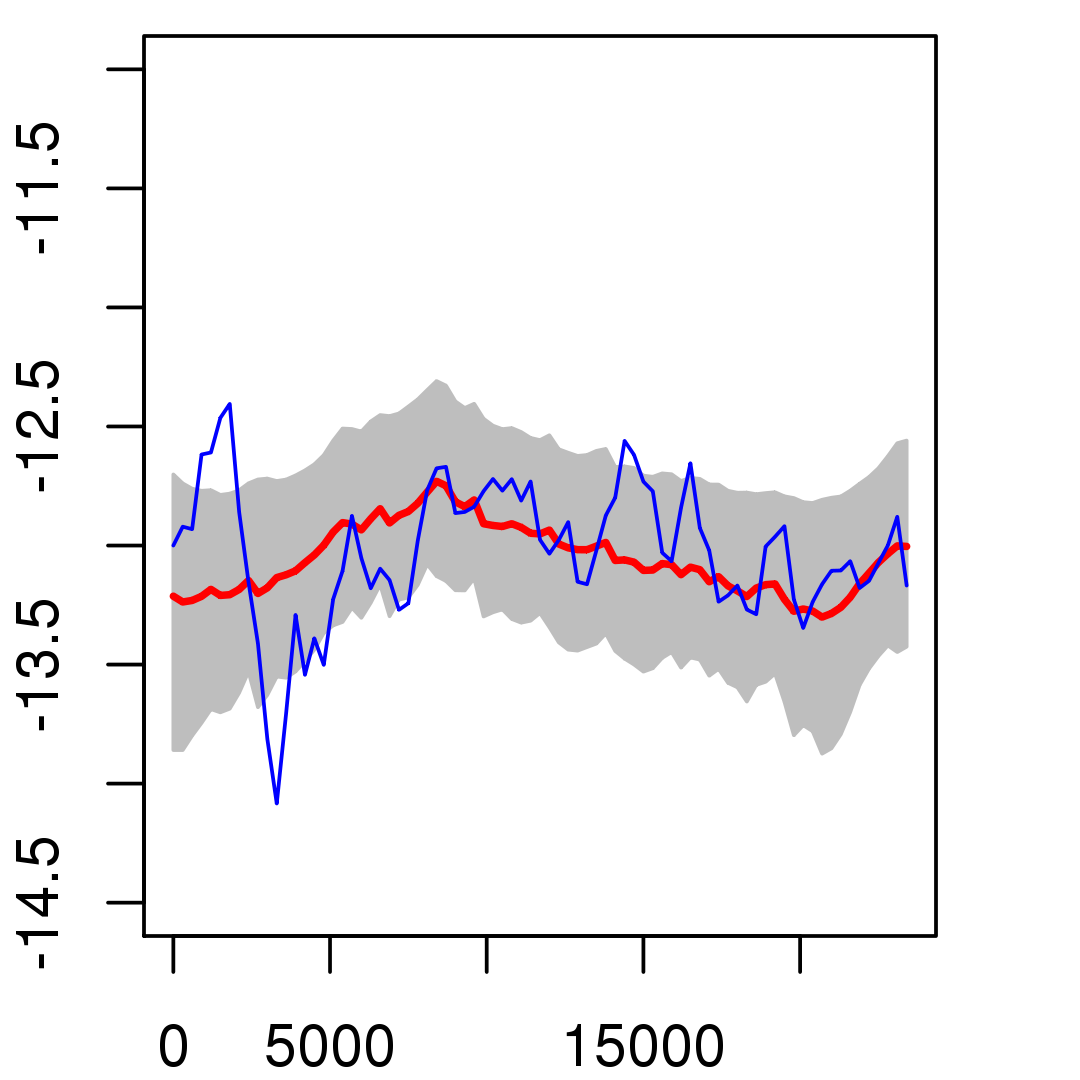
\includegraphics[width=1\linewidth]{results-simulation-10003-bid-ask-noise-plots-VOL-PATHS-microstructure-VOL-PATHS-XI-0-dt-3e05-SDs-0.png}
% 				\end{minipage}
% 			& \begin{minipage}{0.25\textwidth}
% 				\centering
% 				\includegraphics[width=1\linewidth]{{results-simulation-10003-bid-ask-noise-plots-VOL-PATHS-microstructure-VOL-PATHS-XI-2.5e-07-dt-3e05-SDs-0}.png}
% 				\end{minipage}
% 			& \begin{minipage}{0.25\textwidth}
% 				\centering
% 				\includegraphics[width=1\linewidth]{{/home/gdinolov/PDE-solvers/test-sv-sample-4-days/slow-vol-delta-t-300}.pdf}
% 				\end{minipage}  \\
%    %
%           		\begin{sideways} $\Delta = 5$ min, fast \end{sideways}
% 			& \begin{minipage}{0.25\textwidth}
% 				\centering
% 				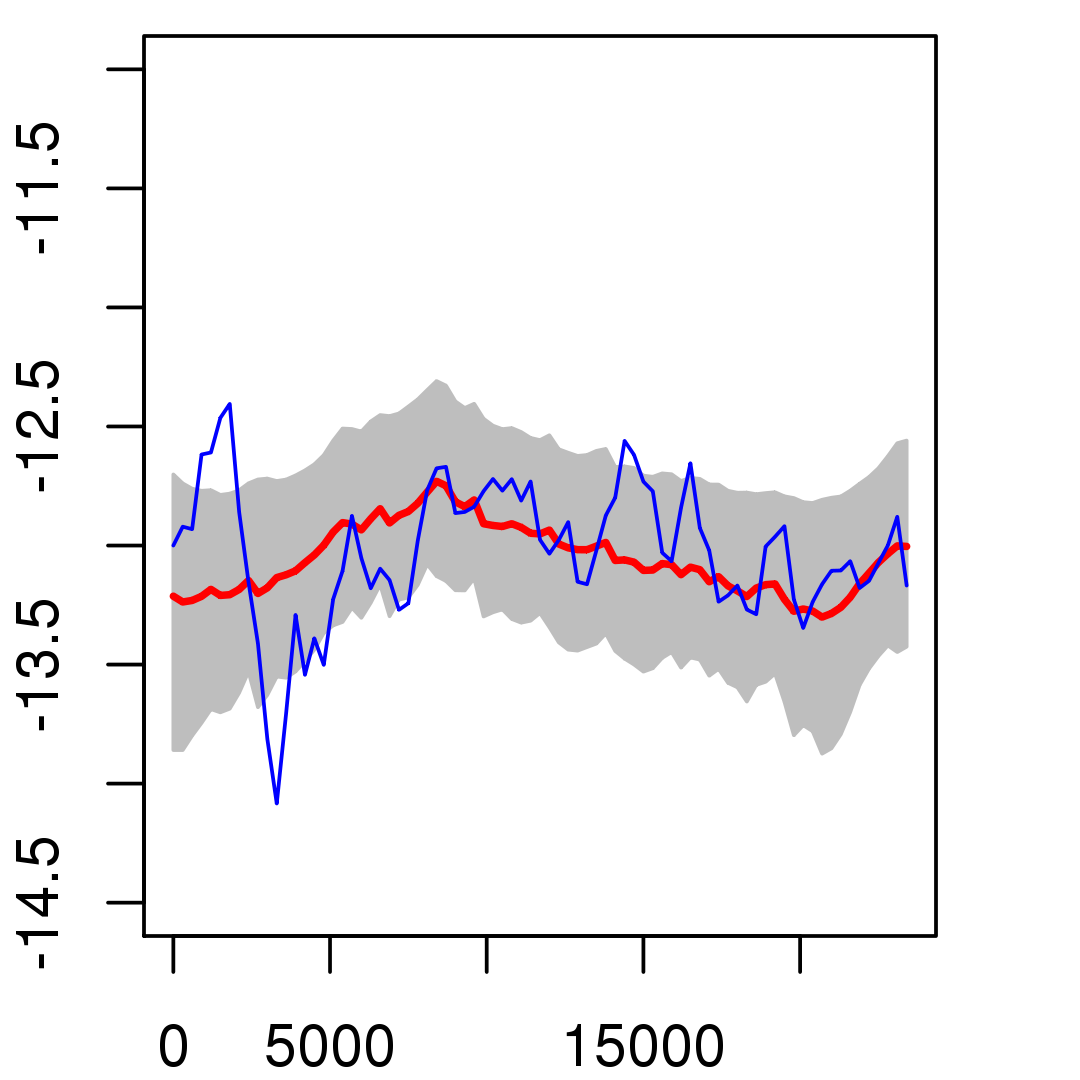
\includegraphics[width=1\linewidth]{results-simulation-10003-bid-ask-noise-plots-VOL-PATHS-microstructure-VOL-PATHS-XI-0-dt-3e05-SDs-0.png}
% 				\end{minipage}
% 			& \begin{minipage}{0.25\textwidth}
% 				\centering
% 				\includegraphics[width=1\linewidth]{{results-simulation-10003-bid-ask-noise-plots-VOL-PATHS-microstructure-VOL-PATHS-XI-2.5e-07-dt-3e05-SDs-0}.png}
% 				\end{minipage}
% 			& \begin{minipage}{0.25\textwidth}
% 				\centering
% 				\includegraphics[width=1\linewidth]{{/home/gdinolov/PDE-solvers/test-sv-sample-4-days/fast-vol-delta-t-300}.pdf}
% 				\end{minipage}  \\
% %
% 		\begin{sideways} $\Delta = 60$ sec, slow \end{sideways}
% 			& \begin{minipage}{0.25\textwidth}
% 				\centering
% 				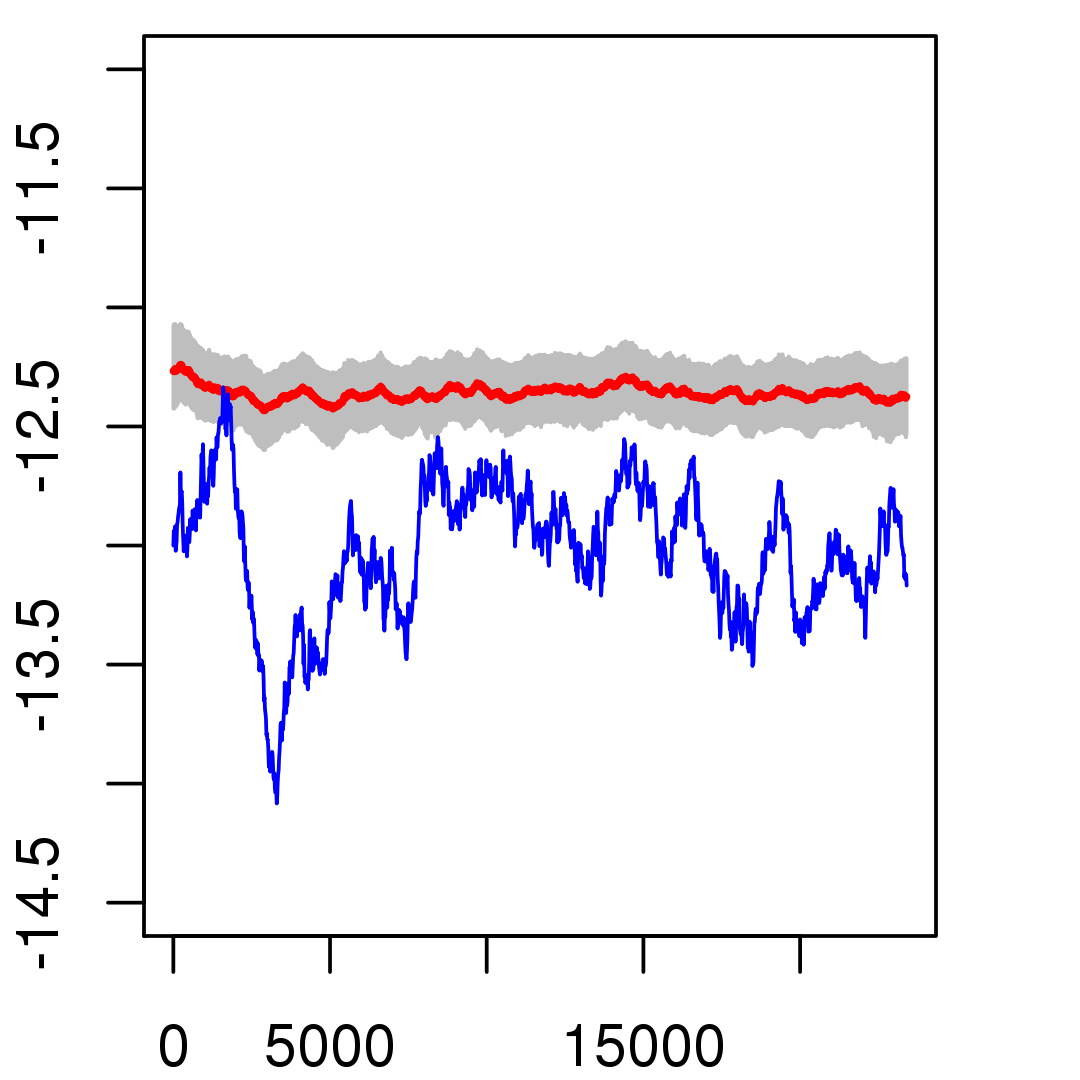
\includegraphics[width=1\linewidth]{results-simulation-10003-bid-ask-noise-plots-VOL-PATHS-microstructure-VOL-PATHS-XI-0-dt-15000-SDs-0.png}
% 				\end{minipage}
% 			& \begin{minipage}{0.25\textwidth}
% 				\centering
% 				\includegraphics[width=1\linewidth]{{results-simulation-10003-bid-ask-noise-plots-VOL-PATHS-microstructure-VOL-PATHS-XI-2.5e-07-dt-15000-SDs-0}.png}
% 				\end{minipage}
% 			& \begin{minipage}{0.25\textwidth}
% 				\centering
% 				\includegraphics[width=1\linewidth]{{/home/gdinolov/PDE-solvers/test-sv-sample-4-days/slow-vol-delta-t-60}.pdf}
% 				\end{minipage}  \\
%    %
%           		\begin{sideways} $\Delta = 60$ sec, fast \end{sideways}
% 			& \begin{minipage}{0.25\textwidth}
% 				\centering
% 				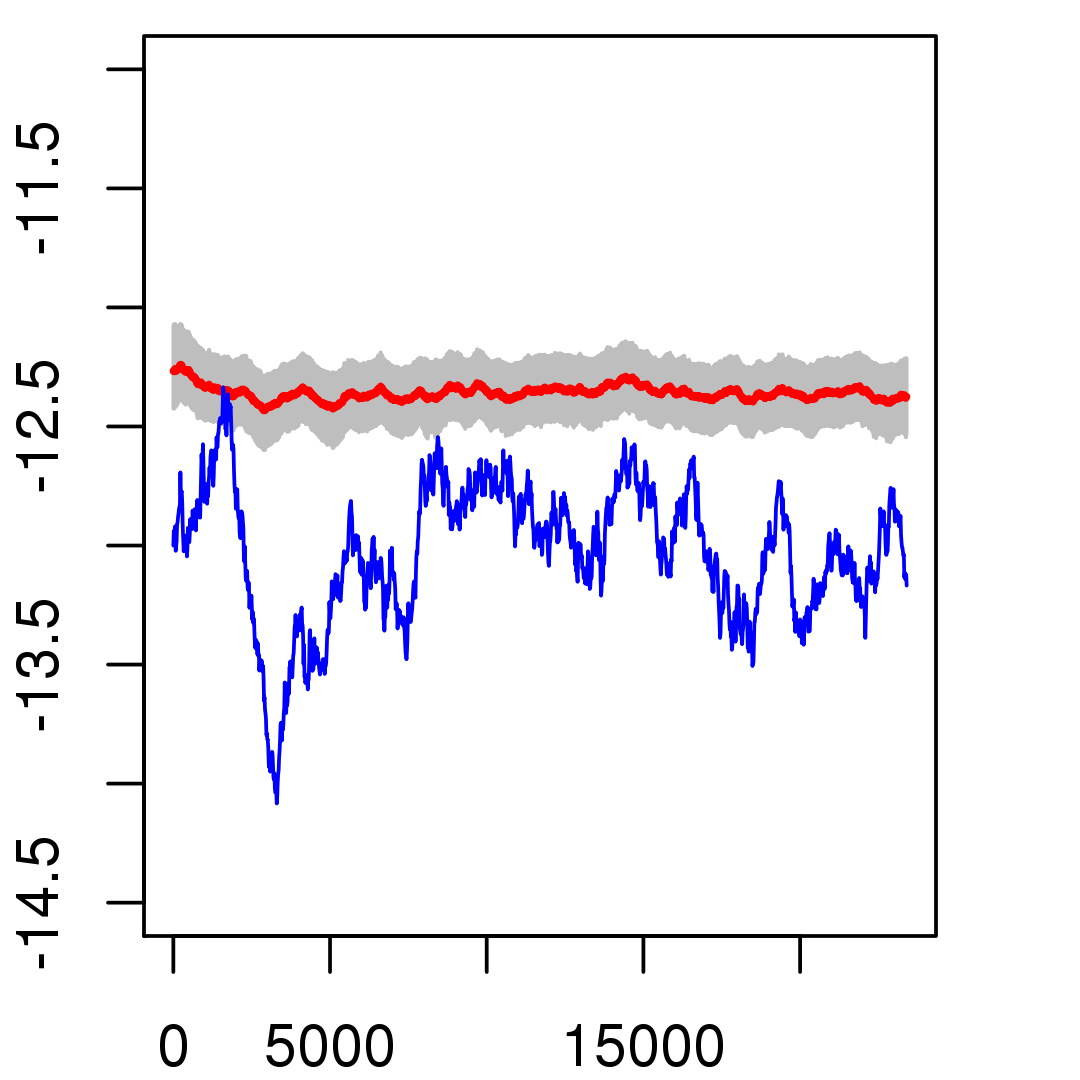
\includegraphics[width=1\linewidth]{results-simulation-10003-bid-ask-noise-plots-VOL-PATHS-microstructure-VOL-PATHS-XI-0-dt-15000-SDs-0.png}
% 				\end{minipage}
% 			& \begin{minipage}{0.25\textwidth}
% 				\centering
% 				\includegraphics[width=1\linewidth]{{results-simulation-10003-bid-ask-noise-plots-VOL-PATHS-microstructure-VOL-PATHS-XI-2.5e-07-dt-15000-SDs-0}.png}
% 				\end{minipage}
% 			& \begin{minipage}{0.25\textwidth}
% 				\centering
% 				\includegraphics[width=1\linewidth]{{/home/gdinolov/PDE-solvers/test-sv-sample-4-days/fast-vol-delta-t-60}.pdf}
% 				\end{minipage}  \\
% %
% 			\begin{sideways} $\Delta = 5$ sec, slow \end{sideways}
% 			& \begin{minipage}{0.25\textwidth}
% 				\centering
%                                 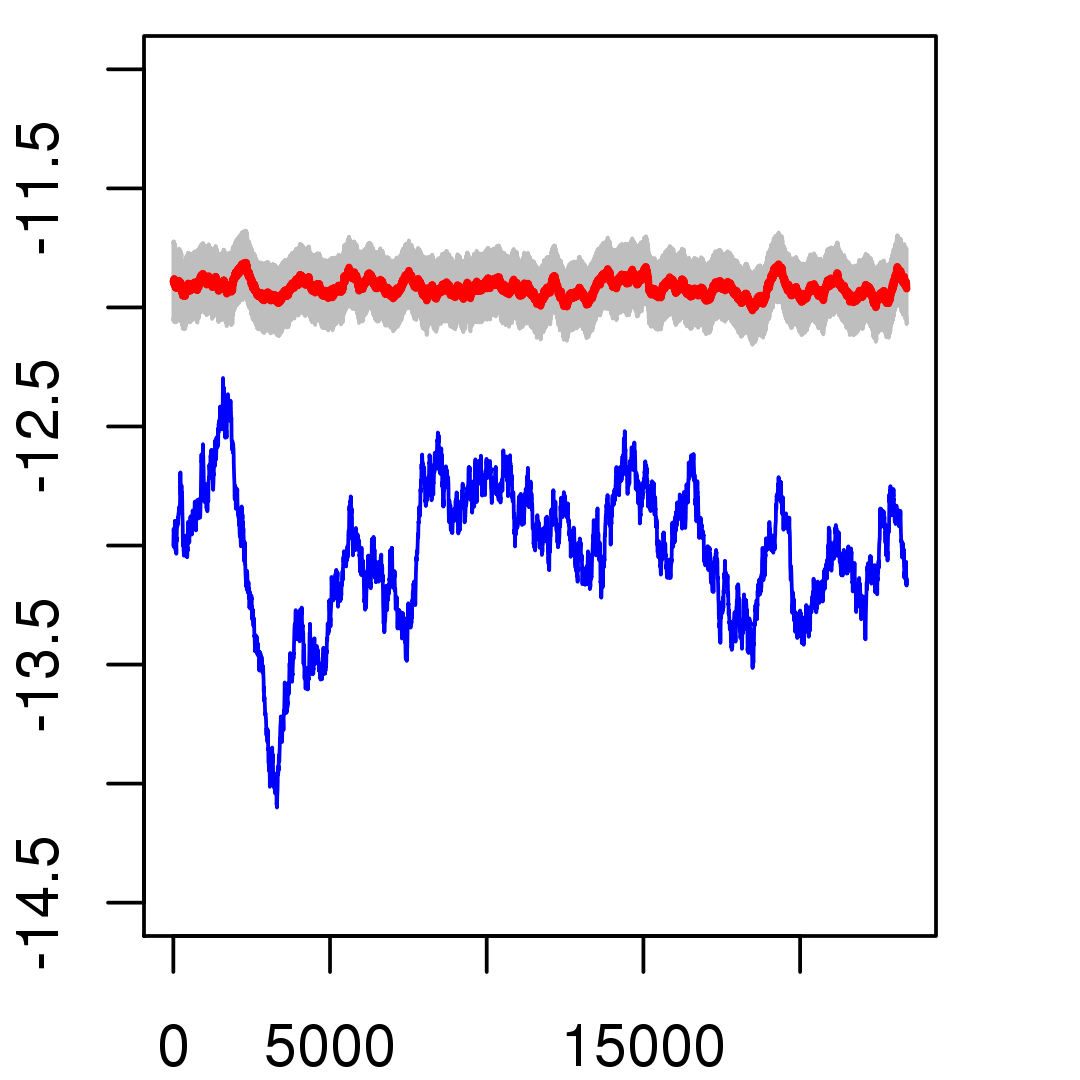
\includegraphics[width=1\linewidth]{results-simulation-10003-bid-ask-noise-plots-VOL-PATHS-microstructure-VOL-PATHS-XI-0-dt-5000-SDs-0.png}
% 				\end{minipage}
% 			& \begin{minipage}{0.25\textwidth}
% 				\centering
%                                 \includegraphics[width=1\linewidth]{{results-simulation-10003-bid-ask-noise-plots-VOL-PATHS-microstructure-VOL-PATHS-XI-2.5e-07-dt-5000-SDs-0}.png}
% 				\end{minipage}
% 			& \begin{minipage}{0.25\textwidth}
% 				\centering
%                                 \includegraphics[width=1\linewidth]{{/home/gdinolov/PDE-solvers/test-sv-sample-4-days/slow-vol-delta-t-30}.pdf}
%                               \end{minipage} \\
%                    %
% 			\begin{sideways} $\Delta = 5$ sec, fast \end{sideways}
% 			& \begin{minipage}{0.25\textwidth}
% 				\centering
%                                 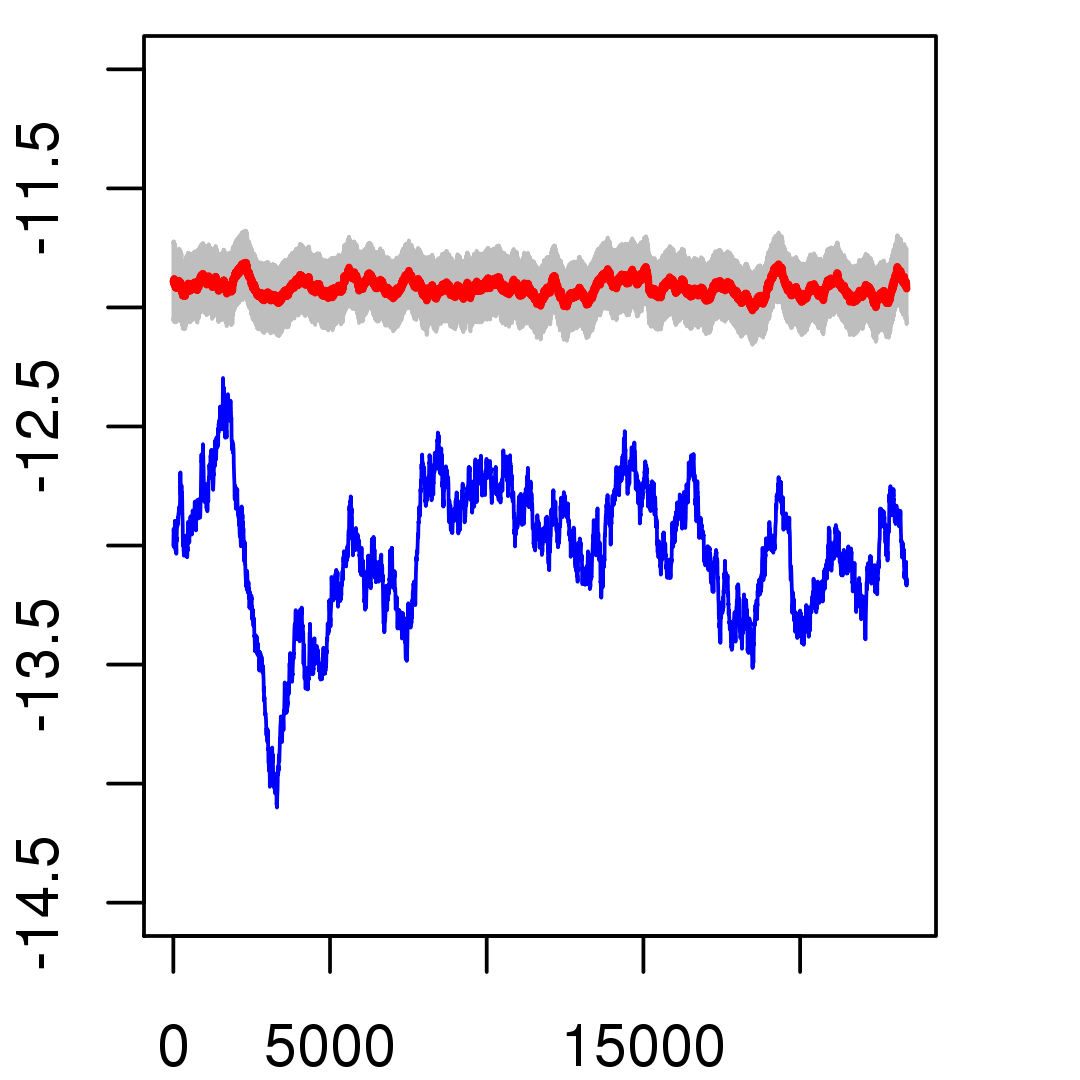
\includegraphics[width=1\linewidth]{results-simulation-10003-bid-ask-noise-plots-VOL-PATHS-microstructure-VOL-PATHS-XI-0-dt-5000-SDs-0.png}
% 				\end{minipage}
% 			& \begin{minipage}{0.25\textwidth}
% 				\centering
%                                 \includegraphics[width=1\linewidth]{{results-simulation-10003-bid-ask-noise-plots-VOL-PATHS-microstructure-VOL-PATHS-XI-2.5e-07-dt-5000-SDs-0}.png}
% 				\end{minipage}
% 			& \begin{minipage}{0.25\textwidth}
% 				\centering
%                                 \includegraphics[width=1\linewidth]{{/home/gdinolov/PDE-solvers/test-sv-sample-4-days/fast-vol-delta-t-30}.pdf}
% 				\end{minipage}
% 	\end{tabular}
% \caption{Log-volatility paths for simulated data. All three inference approaches are applied to the same data set that contains microsructure noise. The miscrostructure noise added in the simulated data is approximately at the level of $\xi^2 = 2.5\cdot 10^{-7}$. Red denotes the posterior mean of the paths, while the gray region denotes the posterior 95\% probability for the log-volatility value. Blue is the true log-volatility signal. We see that when microstructure is ignored ($\xi^2 = 0$), we fail to recover the true signal.}  \label{fig:log-vol-simulation}
% \end{figure}


\begin{figure}[h!]
\centering
\begin{tabular}{m{0.25cm}ccc}
		 & Inference with & Inference with & Inference with \\
		 & $\xi^2 = 0$ & $\xi^2 = 2.5 \cdot 10^{-7}$ & $\xi^2 \mbox{ estimated }$ \\
%
  \begin{sideways} $\hat{\mu}$ \end{sideways}
                 & \begin{minipage}{0.20\textwidth}
                   \centering
                   \includegraphics[width=1\linewidth]{{/home/gdinolov/PDE-solvers/test-sv-sample-4-days/xi-zero-mu-hat}.pdf}
                 \end{minipage} & \begin{minipage}{0.20\textwidth}
                   \centering
                   \includegraphics[width=1\linewidth]{{/home/gdinolov/PDE-solvers/test-sv-sample-4-days/xi-fixed-mu-hat}.pdf}
                 \end{minipage} & \begin{minipage}{0.20\textwidth}
                   \centering
                   \includegraphics[width=1\linewidth]{{/home/gdinolov/PDE-solvers/test-sv-sample-4-days/mu-hat}.pdf}
                 \end{minipage} \\
  \begin{sideways} $\mbox{logit}\left(\frac{\rho+1}{2}\right)$ \end{sideways}
                 & \begin{minipage}{0.20\textwidth}
                   \centering
                   \includegraphics[width=1\linewidth]{{/home/gdinolov/PDE-solvers/test-sv-sample-4-days/xi-zero-rho}.pdf}
                 \end{minipage} & \begin{minipage}{0.20\textwidth}
                   \centering
                   \includegraphics[width=1\linewidth]{{/home/gdinolov/PDE-solvers/test-sv-sample-4-days/xi-fixed-rho}.pdf}
                 \end{minipage} & \begin{minipage}{0.20\textwidth}
                   \centering
                   \includegraphics[width=1\linewidth]{{/home/gdinolov/PDE-solvers/test-sv-sample-4-days/rho}.pdf}
                 \end{minipage} \\
  \begin{sideways} $\log\left(\xi^2\right)$ \end{sideways}
                 & & & \begin{minipage}{0.20\textwidth}
                   \centering
                   \includegraphics[width=1\linewidth]{{/home/gdinolov/PDE-solvers/test-sv-sample-4-days/xi-square}.pdf}
                 \end{minipage}
\end{tabular}
\caption{Posterior density approximations of the observational model
  parameters for simulated data. The black vertical line represents
  the true parameter value. The sampling periods used are: 5 minutes,
  60 seconds, and 10
  seconds.}  \label{fig:observational-parameters-simulated}
\end{figure}


\begin{figure}[h!]
\centering
\begin{tabular}{m{0.25cm}ccc}
		 & Inference with & Inference with & Inference with \\
		 & $\xi^2 = 0$ & $\xi^2 = 2.5 \cdot 10^{-7}$ & $\xi^2 \mbox{ estimated }$ \\
   %    
  \begin{sideways} $\halpha$ \end{sideways}
                 & \begin{minipage}{0.20\textwidth}
                   \centering
                   \includegraphics[width=1\linewidth]{{/home/gdinolov/PDE-solvers/test-sv-sample-4-days/xi-zero-alpha-hat}.pdf}
                 \end{minipage} & \begin{minipage}{0.20\textwidth}
                   \centering
                   \includegraphics[width=1\linewidth]{{/home/gdinolov/PDE-solvers/test-sv-sample-4-days/xi-fixed-alpha-hat}.pdf}
                 \end{minipage} & \begin{minipage}{0.20\textwidth}
                   \centering
                   \includegraphics[width=1\linewidth]{{/home/gdinolov/PDE-solvers/test-sv-sample-4-days/alpha-hat}.pdf}
                 \end{minipage}  \\
                 % 
  \begin{sideways} $\log\left(\htau^2_{\mbox{slow}}\right)$ \end{sideways}
                 & \begin{minipage}{0.20\textwidth}
                   \centering
                   \includegraphics[width=1\linewidth]{{/home/gdinolov/PDE-solvers/test-sv-sample-4-days/xi-zero-tau-square-hat-slow}.pdf}
                 \end{minipage} & \begin{minipage}{0.20\textwidth}
                   \centering
                   \includegraphics[width=1\linewidth]{{/home/gdinolov/PDE-solvers/test-sv-sample-4-days/xi-fixed-tau-square-hat-slow}.pdf}
                 \end{minipage} & \begin{minipage}{0.20\textwidth}
                   \centering
                   \includegraphics[width=1\linewidth]{{/home/gdinolov/PDE-solvers/test-sv-sample-4-days/tau-square-hat-slow}.pdf}
                 \end{minipage}  \\
                 % 
  \begin{sideways} $\log\left(\htau^2_{\mbox{fast}}\right)$ \end{sideways}
                 & \begin{minipage}{0.20\textwidth}
                   \centering
                   \includegraphics[width=1\linewidth]{{/home/gdinolov/PDE-solvers/test-sv-sample-4-days/xi-zero-tau-square-hat-fast}.pdf}
                 \end{minipage} & \begin{minipage}{0.20\textwidth}
                   \centering
                   \includegraphics[width=1\linewidth]{{/home/gdinolov/PDE-solvers/test-sv-sample-4-days/xi-fixed-tau-square-hat-fast}.pdf}
                 \end{minipage} & \begin{minipage}{0.20\textwidth}
                   \centering
                   \includegraphics[width=1\linewidth]{{/home/gdinolov/PDE-solvers/test-sv-sample-4-days/tau-square-hat-fast}.pdf}
                 \end{minipage}  \\
                 % 
  \begin{sideways} $\log\left(\hat{\theta}_{\mbox{slow}}\right)$ \end{sideways}
                 & \begin{minipage}{0.20\textwidth}
                   \centering
                   \includegraphics[width=1\linewidth]{{/home/gdinolov/PDE-solvers/test-sv-sample-4-days/xi-zero-theta-hat-slow}.pdf}
                 \end{minipage} & \begin{minipage}{0.20\textwidth}
                   \centering
                   \includegraphics[width=1\linewidth]{{/home/gdinolov/PDE-solvers/test-sv-sample-4-days/xi-fixed-theta-hat-slow}.pdf}
                 \end{minipage} & \begin{minipage}{0.20\textwidth}
                   \centering
                   \includegraphics[width=1\linewidth]{{/home/gdinolov/PDE-solvers/test-sv-sample-4-days/theta-hat-slow}.pdf}
                 \end{minipage}  \\
                 % 
  \begin{sideways} $\log\left(\hat{\theta}_{\mbox{fast}}\right)$ \end{sideways}
                 & \begin{minipage}{0.20\textwidth}
                   \centering
                   \includegraphics[width=1\linewidth]{{/home/gdinolov/PDE-solvers/test-sv-sample-4-days/xi-zero-theta-hat-fast}.pdf}
                 \end{minipage}
                                  & \begin{minipage}{0.20\textwidth}
                                    \centering
				\includegraphics[width=1\linewidth]{{/home/gdinolov/PDE-solvers/test-sv-sample-4-days/xi-fixed-theta-hat-fast}.pdf}
				\end{minipage}
			& \begin{minipage}{0.20\textwidth}
				\centering
                                \includegraphics[width=1\linewidth]{{/home/gdinolov/PDE-solvers/test-sv-sample-4-days/theta-hat-fast}.pdf}
				\end{minipage} 
\end{tabular}
\caption{Posterior density approximations of volatility model
  parameters for simulated data. The red vertical line represents the
  true parameter value. The sampling periods used are: 5 minutes, 60
  seconds, and 10
  seconds.}  \label{fig:volatility-parameters-simulated}
\end{figure}

In addition to estimating the volatility path, we also investigate the ability of the model to infer model parameters.  In particular, Figure \ref{fig:volatility-parameters-simulated} shows the posterior density estimates for the continuous-time parameters $\hat{\alpha}$, $\hat{\tau}^2$, $\hat{\theta}$ and $\hat{\mu}$ (which are comparable across scales), as well as the posterior distribution for $\xi^2$ (in the case of the third version of the model, which is the only one in which it is estimated from the data).  Note that, when the model is estimated with $\xi^2 = 0$ fixed, the posterior densities for $\halpha$, the mean level of log volatility, show a reduction in variance with increasing sampling frequency:  posterior draws become more centered around a wrong, overestimated value for mean log-volatility level. These results are consistent with those obtained for the volatility path and show that the model fails to capture the constant information content in the data regarding $\halpha$.  We also note that learning $\htau^2$ and $\htheta$ is difficult whether we do or do not include microstructure noise. However, due to the constant information in the data with respect to $\halpha$, the posterior uncertainty for $\htheta$ and $\htau^2$ seems to remain constant even with increasing sampling frequency when $\xi$ is not fixed.

\subsection{Estimating Integrated Variance}

As described in Section \ref{se:computation}, the posterior draws for $\sigma^2_{j}$ allow us to approximate the posterior distributions for the integrated variance of the latent volatility process. In this Section we extend the previous simulation study to compare the 95\% intervals generated by the three versions of our model with those generated from a realized variance estimate.  The literature on realized volatility estimators for high-frequency data is vast (for a review, refer to \cite{pigorsch2012volatility}), but the construction of confidence intervals for the realized volatility estimators can be challenging.  Here we compare the coverage properties of our model-based credible intervals against bootstrap-based confidence intervals of the the kernel-based realized variance estimator introduced by \cite{zhou1996high} and \cite{hansen2006realized}. The idea behind the bootstrapping method is to periodically extend the available data set and randomly reselect a new data set to construct a bootstrap sample (see \cite{hwang2013stationary-bootstrap} for a full description of the procedure).

The results of the comparison are shown in Table \ref{ta:coverage}. The table is constructed using 300 simulated data sets, each corresponding to a single trading day. We compare the percentage of times the 95\% confidence/credible intervals for the integrated variance (IV) estimator covers the true integrated variance value.  A well-calibrated interval will produce a 95\% coverage on average, and we see that the estimator based on our approach where $\xi^2$ is fully estimated preforms very well, both when compared to $\xi^2 =0$, $\xi^2 = 2.5 \cdot 10^{-7}$, and when compared to the kernel-based estimator.

\begin{table}[h]
\begin{center}
\begin{tabular}{l|ccccc}
Sampling period   &   5 min  &	60 sec 	&   30 sec   &   15 sec & 5 sec  \\ \hline \hline
Inference with $\xi^2 = 0$  &  93  &  72  &   28  &	 3 & 0 \\
Inference with $\xi^2 = 2.5 \cdot 10^{-7}$ & 95 & 79 & 57 & 23 & 0 \\
Inference with $\xi^2$ estimated & 95 & 91 & 92 & 96 & 97  \\ \hline
Inference with kernel-based estimator &  53 & 51 & 48 & 59  & 76
\end{tabular}
\caption{Coverage table comparing the percentage of covered integrated variance levels by 95\% confidence/credible intervals of our estimator and a kernel-based estimator.}\label{ta:coverage}
\end{center}
\end{table}

%\newpage
\subsection{ Effect of microstructure noise and sampling frequency on estimates: market data }

We perform an analysis for real market data, which consists of a single day of midpoint spot prices of Apple Inc. (NASDAQ:AAPL) on March $6^{th}$, 2014, printed on the millisecond from the NYSE TAQ data set.  Our a priori distribution for the bid-ask spread driving microstructure noise is centered on \$0.1 as with the simulation data. All other priors are the same as in Section \ref{se:simulation-results}.  The estimated volatility paths are shown in Figure \ref{fig:log-vol-real}.  In the case where $\xi^2 = 0$, the model estimates the volatility signal to be, on average, higher than in the cases where $\xi^2 > 0$, which is also seen in the posterior means estimates of $\halpha$ in Figure \ref{fig:posterior-parameters-real}. This is consistent with the simulation-study results, where the $\xi^2 = 0$ model attributes microstructure noise to the log-volatility signal.

\begin{figure}
	\centering
	\begin{tabular}{m{0.25cm}ccc}
		 & Inference with & Inference with & Inference with \\
		 & $\xi^2 = 0$ & $\xi^2 = 2.5 \cdot 10^{-7}$ & $\xi^2 \mbox{ estimated }$ \\
%
		\begin{sideways} $\Delta = 5$ min \end{sideways}
			& \begin{minipage}{0.25\textwidth}
				\centering
				\includegraphics[width=1\linewidth]{/home/gdinolov/PDE-solvers/src/SV-with-leverage/paper-revisions-7-11-2016/results-real-data-plots-VOL-PATHS-microstructure-VOL-PATHS-XI-0-dt-3e05-SDs-0.png}
				\end{minipage}
			& \begin{minipage}{0.25\textwidth}
				\centering
				\includegraphics[width=1\linewidth]{{/home/gdinolov/PDE-solvers/src/SV-with-leverage/paper-revisions-7-11-2016/results-real-data-plots-VOL-PATHS-microstructure-VOL-PATHS-XI-2.5e-07-dt-3e05-SDs-0}.png}
				\end{minipage}
			& \begin{minipage}{0.25\textwidth}
				\centering
				\includegraphics[width=1\linewidth]{/home/gdinolov/PDE-solvers/src/SV-with-leverage/paper-revisions-7-11-2016/results-real-data-plots-VOL-PATHS-microstructure-VOL-PATHS-XI-Inf-dt-3e05-SDs-0.png}
				\end{minipage}  \\
%
		\begin{sideways} $\Delta = 15$ sec \end{sideways}
			& \begin{minipage}{0.25\textwidth}
				\centering
				\includegraphics[width=1\linewidth]{/home/gdinolov/PDE-solvers/src/SV-with-leverage/paper-revisions-7-11-2016/results-real-data-plots-VOL-PATHS-microstructure-VOL-PATHS-XI-0-dt-15000-SDs-0.png}
				\end{minipage}
			& \begin{minipage}{0.25\textwidth}
				\centering
				\includegraphics[width=1\linewidth]{{/home/gdinolov/PDE-solvers/src/SV-with-leverage/paper-revisions-7-11-2016/results-real-data-plots-VOL-PATHS-microstructure-VOL-PATHS-XI-2.5e-07-dt-15000-SDs-0}.png}
				\end{minipage}
			& \begin{minipage}{0.25\textwidth}
				\centering
				\includegraphics[width=1\linewidth]{/home/gdinolov/PDE-solvers/src/SV-with-leverage/paper-revisions-7-11-2016/results-real-data-plots-VOL-PATHS-microstructure-VOL-PATHS-XI-Inf-dt-15000-SDs-0.png}
				\end{minipage}  \\
%
			\begin{sideways} $\Delta = 5$ sec \end{sideways}
			& \begin{minipage}{0.25\textwidth}
				\centering
				\includegraphics[width=1\linewidth]{/home/gdinolov/PDE-solvers/src/SV-with-leverage/paper-revisions-7-11-2016/results-real-data-plots-VOL-PATHS-microstructure-VOL-PATHS-XI-0-dt-5000-SDs-0.png}
				\end{minipage}
			& \begin{minipage}{0.25\textwidth}
				\centering
				\includegraphics[width=1\linewidth]{{/home/gdinolov/PDE-solvers/src/SV-with-leverage/paper-revisions-7-11-2016/results-real-data-plots-VOL-PATHS-microstructure-VOL-PATHS-XI-2.5e-07-dt-5000-SDs-0}.png}
				\end{minipage}
			& \begin{minipage}{0.25\textwidth}
				\centering
				\includegraphics[width=1\linewidth]{/home/gdinolov/PDE-solvers/src/SV-with-leverage/paper-revisions-7-11-2016/results-real-data-plots-VOL-PATHS-microstructure-VOL-PATHS-XI-Inf-dt-5000-SDs-0.png}
				\end{minipage}  \\
%%
%			\begin{sideways} $\Delta = 1$ sec \end{sideways}
%			& \begin{minipage}{0.25\textwidth}
%				\centering
%				\includegraphics[width=1\linewidth]{results/real-data/plots/VOL-PATHS/microstructure-VOL-PATHS-XI-0-dt-1000-SDs-0.png}
%				\end{minipage}
%			& \begin{minipage}{0.25\textwidth}
%				\centering
%				\includegraphics[width=1\linewidth]{results/real-data/plots/VOL-PATHS/microstructure-VOL-PATHS-XI-1e-06-dt-1000-SDs-0.png}
%				\end{minipage}
%			& \begin{minipage}{0.25\textwidth}
%				\centering
%				\includegraphics[width=1\linewidth]{results/real-data/plots/VOL-PATHS/microstructure-VOL-PATHS-XI-Inf-dt-1000-SDs-0.png}
%				\end{minipage}
	\end{tabular}
	\caption{Log-volatility paths for the AAPL 03/06/2014 data. Red denotes the posterior mean of the paths, while the gray region denotes the posterior 95\% probability for the log-volatility value.}
	\label{fig:log-vol-real}
\end{figure}

Figure \ref{fig:posterior-parameters-real} shows the posterior distributions for the model parameters.   Note that the posterior for $\xi^2$ is centered around $8 \cdot 10^{-9}$ -- two orders of magnitude smaller than the prior center of $2.7 \cdot 10^{-7}$. This value of the posterior mean is roughly equivalent to a bid-ask spread of \$0.01, which is reasonable for a highly-traded stock like AAPL.  Furthermore, note that fixing $\xi^2 = 2.5\cdot 10^{-7}$ compared to treaing $\xi^2$ as an unknown parameter, leads to volatility paths that are smoother and have greater coherence in posterior estimates of the model parameters across sampling periods.  This is especially true for $\htheta$, since the closer the log-volatility process is to being discontinuous, the shorter its timescale must be.  We thus see the obvious trade-off when specifying $\xi^2$: if $\xi^2$ is too large, we run the risk of over-smoothing; if $\xi^2$ is too small, we confound the effects of noise with those of the volatility process.

\begin{figure}[h!]
	\centering
%
	\begin{tabular}{m{0.25cm}ccc}
		 & Inference with & Inference with & Inference with \\
		 & $\xi^2 = 0$ & $\xi^2 = 1 \cdot 10^{-6}$ & $\xi^2 \mbox{ estimated }$ \\
%
		\begin{sideways} $\halpha$ \end{sideways}
n			& \begin{minipage}{0.20\textwidth}
				\centering
				\includegraphics[width=1\linewidth]{/home/gdinolov/PDE-solvers/src/SV-with-leverage/paper-revisions-7-11-2016/results-real-data-plots-ALPHAS-microstructure-ALPHA-XI-0-SDs-0.pdf}
				\end{minipage}
			& \begin{minipage}{0.20\textwidth}
				\centering
				\includegraphics[width=1\linewidth]{{/home/gdinolov/PDE-solvers/src/SV-with-leverage/paper-revisions-7-11-2016/results-real-data-plots-ALPHAS-microstructure-ALPHA-XI-2.5e-07-SDs-0}.pdf}
				\end{minipage}
			& \begin{minipage}{0.20\textwidth}
				\centering
				\includegraphics[width=1\linewidth]{/home/gdinolov/PDE-solvers/src/SV-with-leverage/paper-revisions-7-11-2016/results-real-data-plots-ALPHAS-microstructure-ALPHA-XI-Inf-SDs-0.pdf}
				\end{minipage}  \\
%
		\begin{sideways} $\htau^2$ \end{sideways}
			& \begin{minipage}{0.20\textwidth}
				\centering
				\includegraphics[width=1\linewidth]{/home/gdinolov/PDE-solvers/src/SV-with-leverage/paper-revisions-7-11-2016/results-real-data-plots-TAUS-SQ-microstructure-TAU-SQ-XI-0-SDs-0.pdf}
				\end{minipage}
			& \begin{minipage}{0.20\textwidth}
				\centering
				\includegraphics[width=1\linewidth]{{/home/gdinolov/PDE-solvers/src/SV-with-leverage/paper-revisions-7-11-2016/results-real-data-plots-TAUS-SQ-microstructure-TAU-SQ-XI-2.5e-07-SDs-0}.pdf}
				\end{minipage}
			& \begin{minipage}{0.20\textwidth}
				\centering
				\includegraphics[width=1\linewidth]{/home/gdinolov/PDE-solvers/src/SV-with-leverage/paper-revisions-7-11-2016/results-real-data-plots-TAUS-SQ-microstructure-TAU-SQ-XI-Inf-SDs-0.pdf}
				\end{minipage}  \\
%
			\begin{sideways} $\hat{\theta}$ \end{sideways}
			& \begin{minipage}{0.20\textwidth}
				\centering
				\includegraphics[width=1\linewidth]{/home/gdinolov/PDE-solvers/src/SV-with-leverage/paper-revisions-7-11-2016/results-real-data-plots-PHIS-microstructure-PHI-XI-0-SDs-0.pdf}
				\end{minipage}
			& \begin{minipage}{0.20\textwidth}
				\centering
				\includegraphics[width=1\linewidth]{{/home/gdinolov/PDE-solvers/src/SV-with-leverage/paper-revisions-7-11-2016/results-real-data-plots-PHIS-microstructure-PHI-XI-2.5e-07-SDs-0}.pdf}
				\end{minipage}
			& \begin{minipage}{0.20\textwidth}
				\centering
				\includegraphics[width=1\linewidth]{/home/gdinolov/PDE-solvers/src/SV-with-leverage/paper-revisions-7-11-2016/results-real-data-plots-PHIS-microstructure-PHI-XI-Inf-SDs-0.pdf}
				\end{minipage}  \\
%
			\begin{sideways} $\hat{\mu}$ \end{sideways}
			& \begin{minipage}{0.20\textwidth}
				\centering
				\includegraphics[width=1\linewidth]{/home/gdinolov/PDE-solvers/src/SV-with-leverage/paper-revisions-7-11-2016/results-real-data-plots-MUS-microstructure-MU-XI-0-SDs-0.pdf}
				\end{minipage}
			& \begin{minipage}{0.20\textwidth}
				\centering
				\includegraphics[width=1\linewidth]{{/home/gdinolov/PDE-solvers/src/SV-with-leverage/paper-revisions-7-11-2016/results-real-data-plots-MUS-microstructure-MU-XI-2.5e-07-SDs-0}.pdf}
				\end{minipage}
			&\begin{minipage}{0.20\textwidth}
				\centering
				\includegraphics[width=1\linewidth]{/home/gdinolov/PDE-solvers/src/SV-with-leverage/paper-revisions-7-11-2016/results-real-data-plots-MUS-microstructure-MU-XI-Inf-SDs-0.pdf}
				\end{minipage} \\
%
          \begin{sideways} $\xi^2$ \end{sideways}
			&
			&
			&\begin{minipage}{0.20\textwidth}
				\centering
				\includegraphics[width=1\linewidth]{/home/gdinolov/PDE-solvers/src/SV-with-leverage/paper-revisions-7-11-2016/results-real-data-plots-microstructure-XI.pdf}
				\end{minipage}
	\end{tabular}
	\caption{Posterior density approximations of model parameters
          for the AAPL 03/06/2014 data. The sampling periods used are:
          5 minutes \usebox{\legendLineOne}, 30 seconds
          \usebox{\legendLineTwo}, 15 seconds
          \usebox{\legendLineThree}, 5 seconds
          \usebox{\legendLineFour}, and 1 second
          \usebox{\legendLineFive}. Vertical red lines represent prior
          mean for the given parameters.}
	\label{fig:posterior-parameters-real}
\end{figure}

\subsection{Effect of timescale of inertia on estimates of $\halpha$}\label{se:effect-timescale}

To illustrate the discussion in Section \ref{effect-mean-reverting-rate} on the effect of the log-volatility timescale on our method's ability to learn $\halpha$, we examine the posterior uncertainty for $\halpha$ under two scenarios: (1) increasing sample size $N$ by decreasing the sampling period $\Delta$, and (2) increasing $N$ by increasing the observational period $T$ while keeping $\Delta$ constant. The same simulated dataset is used in both (1) and (2), with $1/\htheta = 15 \mbox{ min}$, such that $\htheta \Delta \leq 1$ and the approximation for the posterior variance of $\halpha$ in \eqref{var_alpha_n2} is applicable.
\begin{figure}[h!]
\centering
\begin{tabular}{cc}
			\begin{minipage}{0.45\textwidth}
				\centering
				\includegraphics[width=1\linewidth]{/home/gdinolov/PDE-solvers/src/SV-with-leverage/paper-revisions-7-11-2016/results-simulation-10013-bid-ask-noise-plots-ALPHAS-microstructure-ALPHA-XI-Inf-SDs-0.pdf}
			\end{minipage}
			& \begin{minipage}{0.45\textwidth}
				\centering
				\includegraphics[width=1\linewidth]{/home/gdinolov/PDE-solvers/src/SV-with-leverage/paper-revisions-7-11-2016/alphas-increasing-T.pdf}
				\end{minipage}
\end{tabular}
\caption{Posterior densities of $\halpha$ for two data sets examined under scenarios of increasing sample size $N$ by decreasing $\Delta$ (left) and increasing $N$ by increasing the observational duration $T$ (right). The same data set was used for both cases, where $1/\htheta = 15\, \mbox{min}$ so that $\htheta \Delta \leq 1$ for all posterior samples. The red vertical line signifies the true $\halpha$ value used in the data-generation process. For a fixed $T$ and decreasing $\Delta$ (left) [1 minute \usebox{\legendLineOne}, 30 seconds \usebox{\legendLineTwo}, 15 seconds \usebox{\legendLineThree}, 5 seconds \usebox{\legendLineFour}] the posterior variance of $\halpha$ stays approximately the same. For a fixed $\Delta$ and increasing $T$ [65 minutes \usebox{\legendLineOne}, 130 minutes \usebox{\legendLineTwo}, 195 minutes \usebox{\legendLineThree}, 260 minutes \usebox{\legendLineFour}, 325 minutes \usebox{\legendLineFive}, and 390 \usebox{\legendLineTwo} minutes], the posterior variance of $\halpha$ tends to decrease.}\label{fig:different-phi}
\end{figure}

Under scenario (1), we consider the entire data set and estimate $\halpha$ with $\Delta = 1 \mbox{ min}$, $30 \mbox{ sec}$, $15 \mbox{ sec},$ and $5 \mbox{ sec}$. The posterior distributions for $\halpha$ are shown in the left panel of Figure \ref{fig:different-phi}. We see that the posterior uncertainty for $\halpha$ remains the same with increasing number of intraperiod samples, as suggested by the analysis in Section \ref{effect-mean-reverting-rate}. Under scenario (2), we fix $\Delta = 1 \mbox{ min}$ and increase sample sizes by increasing the observational period $T$, using the first 1/6 (65 min) of the data, the first 2/6 (130 min) of the data, and so on through the entirety of the data (390 min). The right panel of Figure \ref{fig:different-phi} shows the posterior densities for $\halpha$ under this regime. Confirming the discussion in Section \ref{effect-mean-reverting-rate}, we tend to see a decreasing posterior variance for $\halpha$ with increasing observational duration, but not when the sampling frequency increases.  The important takeaway point is that a dataset covering a finite observational period contains a finite amount of information, no matter now finely the observational period is sampled.

%When estimating model parameters, the common intuition is that an increase in sample size leads to a decrease in posterior uncertainty. When dealing with the estimation of stochastic volatility models for high-frequency data, one may be prone to apply this thinking when the sample size is increased by obtaining move frequent price path samples for a fixed observational period. However, as discussed in Section \ref{effect-mean-reverting-rate} and shown in the two scenarios above, in the case where the volatility process has a finite non-zero mean-reversion timescale (as is the case for the OU-process), an increase in the number of intraperiod observations does not add information about the mean-level of the process. Rather, the posterior uncertainty for this model parameter can only be decreased by increasing how long we observe the process. The important takeaway point is that a dataset covering a finite observational period contains a finite amount of information, no matter now finely the observational period is sampled.

\section{Conclusion}

In this paper we have outlined a discrete-time stochastic volatility model for high-frequency data. The model and the algorithm used to estimate it are designed to be coherent across all sampling frequencies. To this end, we elicit priors on the parameters of the continuous-time version of our model and transform them to the discrete-time scale. Both simulation and real data results show that adding the microstructure term in the standard stochastic volatility formulation allows one to fit such models to high-frequency data and extract the log-volatility signal from noisy observations. However, having a good prior estimate of the noise level is an important specification, since attributing some fluctuations in the observed log volatility to microstructure noise has a smoothing effect on the reconstructed log volatility paths. Finally, simulation studies show that the integrated variance estimator derived from our model is well-calibrated and outperforms current kernel-based realized volatility estimators.


% %% SIM 4
% \begin{figure}
%   \centering
%   \begin{tabular}{cc}
%     \begin{minipage}{0.45\textwidth}
%       \centering
%       \includegraphics[width=1\linewidth]{../results-simulated-data/simulation-4/bid-ask-noise/tau-sq-hat-fast-densities.png}
%     \end{minipage}
%     & \begin{minipage}{0.45\textwidth}
%       \centering
%       \includegraphics[width=1\linewidth]{../results-simulated-data/simulation-4/bid-ask-noise/tau-sq-hat-slow-densities.png}
%       \end{minipage} \\
%     \begin{minipage}{0.45\textwidth}
%       \centering
%       \includegraphics[width=1\linewidth]{../results-simulated-data/simulation-4/bid-ask-noise/theta-hat-fast-densities.png}
%     \end{minipage}
%     & \begin{minipage}{0.45\textwidth}
%       \centering
%       \includegraphics[width=1\linewidth]{../results-simulated-data/simulation-4/bid-ask-noise/theta-hat-slow-densities.png}
%     \end{minipage} \\
%     \begin{minipage}{0.45\textwidth}
%       \centering
%       \includegraphics[width=1\linewidth]{../results-simulated-data/simulation-4/bid-ask-noise/rho-densities.png}
%     \end{minipage}
%     & \begin{minipage}{0.45\textwidth}
%       \centering
%       \includegraphics[width=1\linewidth]{../results-simulated-data/simulation-4/bid-ask-noise/alpha-hat-densities.png}
%     \end{minipage}
%   \end{tabular}
%   \caption{Estimating parameters freely with Data Set 4.}
% \end{figure}

% \begin{figure}
%   \centering
%   \begin{tabular}{c}
%     \begin{minipage}{0.80\textwidth}
%       \centering
%       \includegraphics[height=0.5\linewidth]{../results-simulated-data/simulation-4/bid-ask-noise/timeseries-5000.png}
%     \end{minipage} \\
%     \begin{minipage}{0.80\textwidth}
%       \centering
%       \includegraphics[height=0.5\linewidth]{../results-simulated-data/simulation-4/bid-ask-noise/timeseries-1000.png}
%     \end{minipage} \\
%     \begin{minipage}{0.80\textwidth}
%       \centering
%       \includegraphics[height=0.5\linewidth]{../results-simulated-data/simulation-4/bid-ask-noise/timeseries-200.png}
%     \end{minipage}
%   \end{tabular}
%   \caption{Estimating vol paths freely with Data Set 4.}
% \end{figure}

% %% SIM 4
% %% sim 4 fixed rho
% \begin{figure}
%   \centering
%   \begin{tabular}{cc}
%     \begin{minipage}{0.45\textwidth}
%       \centering
%       \includegraphics[width=1\linewidth]{../results-simulated-data/simulation-4/bid-ask-noise/fixed-rho/tau-sq-hat-fast-densities.png}
%     \end{minipage}
%     & \begin{minipage}{0.45\textwidth}
%       \centering
%       \includegraphics[width=1\linewidth]{../results-simulated-data/simulation-4/bid-ask-noise/fixed-rho/tau-sq-hat-slow-densities.png}
%       \end{minipage} \\
%     \begin{minipage}{0.45\textwidth}
%       \centering
%       \includegraphics[width=1\linewidth]{../results-simulated-data/simulation-4/bid-ask-noise/fixed-rho/theta-hat-fast-densities.png}
%     \end{minipage}
%     & \begin{minipage}{0.45\textwidth}
%       \centering
%       \includegraphics[width=1\linewidth]{../results-simulated-data/simulation-4/bid-ask-noise/fixed-rho/theta-hat-slow-densities.png}
%     \end{minipage} \\
%     \begin{minipage}{0.45\textwidth}
%       \centering
%       \includegraphics[width=1\linewidth]{../results-simulated-data/simulation-4/bid-ask-noise/fixed-rho/rho-densities.png}
%     \end{minipage}
%     & \begin{minipage}{0.45\textwidth}
%       \centering
%       \includegraphics[width=1\linewidth]{../results-simulated-data/simulation-4/bid-ask-noise/fixed-rho/alpha-hat-densities.png}
%     \end{minipage}
%   \end{tabular}
%   \caption{Estimating parameters freely with Data Set 4 with fixe rho}
% \end{figure}

% \begin{figure}
%   \centering
%   \begin{tabular}{c}
%     \begin{minipage}{0.80\textwidth}
%       \centering
%       \includegraphics[height=0.5\linewidth]{../results-simulated-data/simulation-4/bid-ask-noise/fixed-rho/timeseries-60000.png}
%     \end{minipage} \\
%     \begin{minipage}{0.80\textwidth}
%       \centering
%       \includegraphics[height=0.5\linewidth]{../results-simulated-data/simulation-4/bid-ask-noise/fixed-rho/timeseries-30000.png}
%     \end{minipage} \\
%     \begin{minipage}{0.80\textwidth}
%       \centering
%       \includegraphics[height=0.5\linewidth]{../results-simulated-data/simulation-4/bid-ask-noise/fixed-rho/timeseries-5000.png}
%     \end{minipage}
%   \end{tabular}
%   \caption{Estimating vol paths freely with Data Set 4 with fixed rho}
% \end{figure}


% %% SIM 5
% \begin{figure}
%   \centering
%   \begin{tabular}{cc}
%     \begin{minipage}{0.45\textwidth}
%       \centering
%       \includegraphics[width=1\linewidth]{../results-simulated-data/simulation-5/bid-ask-noise/tau-sq-hat-fast-densities.png}
%     \end{minipage}
%     & \begin{minipage}{0.45\textwidth}
%       \centering
%       \includegraphics[width=1\linewidth]{../results-simulated-data/simulation-5/bid-ask-noise/tau-sq-hat-slow-densities.png}
%       \end{minipage} \\
%     \begin{minipage}{0.45\textwidth}
%       \centering
%       \includegraphics[width=1\linewidth]{../results-simulated-data/simulation-5/bid-ask-noise/theta-hat-fast-densities.png}
%     \end{minipage}
%     & \begin{minipage}{0.45\textwidth}
%       \centering
%       \includegraphics[width=1\linewidth]{../results-simulated-data/simulation-5/bid-ask-noise/theta-hat-slow-densities.png}
%     \end{minipage} \\
%     \begin{minipage}{0.45\textwidth}
%       \centering
%       \includegraphics[width=1\linewidth]{../results-simulated-data/simulation-5/bid-ask-noise/rho-densities.png}
%     \end{minipage}
%     & \begin{minipage}{0.45\textwidth}
%       \centering
%       \includegraphics[width=1\linewidth]{../results-simulated-data/simulation-5/bid-ask-noise/alpha-hat-densities.png}
%     \end{minipage}
%   \end{tabular}
%   \caption{Estimating parameters freely with Data Set 5, switching $\rho$.}
% \end{figure}

% \begin{figure}
%   \centering
%   \begin{tabular}{c}
%     \begin{minipage}{0.80\textwidth}
%       \centering
%       \includegraphics[height=0.5\linewidth]{../results-simulated-data/simulation-5/bid-ask-noise/timeseries-60000.png}
%     \end{minipage} \\
%     \begin{minipage}{0.80\textwidth}
%       \centering
%       \includegraphics[height=0.5\linewidth]{../results-simulated-data/simulation-5/bid-ask-noise/timeseries-30000.png}
%     \end{minipage} \\
%     \begin{minipage}{0.80\textwidth}
%       \centering
%       \includegraphics[height=0.5\linewidth]{../results-simulated-data/simulation-5/bid-ask-noise/timeseries-5000.png}
%     \end{minipage}
%   \end{tabular}
%   \caption{Estimating vol paths freely with Data Set 5, switching $\rho$..}
% \end{figure}


